% =====================================================================
%  Mecánica I · Tema 1
%  La Mecánica Newtoniana. Cinemática de una partícula en el espacio
%  Compilar:  latexmk -lualatex tema1.tex
% =====================================================================
\documentclass[11pt,a4paper,twoside]{article}
\usepackage{estilo-oscuro}

\renewcommand{\cabeceraimpar}{Tema 1 · Cinemática de una partícula en el espacio}
\renewcommand{\cabecerapar}{Mecánica I}

\hypersetup{pdftitle={Tema 1. La Mecánica Newtoniana. Cinemática de una partícula en el espacio},
  pdfauthor={Daniel Martín Guerrero},pdfsubject={Mecánica I}}

\begin{document}

% =====================================================================
%  PORTADA
% =====================================================================
\begin{titlepage}
\newgeometry{left=27mm,right=27mm,top=20mm,bottom=20mm}
\pagecolor{fondo}\color{texto}
\centering

\includegraphics[width=0.30\textwidth]{figs/logo_usal.png}\par
\vspace{6mm}
{\color{tenue!60}\rule{\textwidth}{0.4pt}}\par
\vspace{4mm}
{\small\color{tenue}\textls[180]{\textsc{Facultad de Ciencias}}\quad·\quad
 \textls[180]{\textsc{Grado en Física}}}\par
\vspace{13mm}
{\color{cian}\textls[220]{\textsc{Mecánica I}}}\par
\vspace{2.2mm}
{\small\color{tenue}\textls[200]{\textsc{Tema 1}}}\par
\vspace{9mm}
{\fontsize{29}{31}\selectfont\bfseries Cinemática de una partícula\\[1mm] en el espacio\par}
\vspace{7mm}
{\color{tenue}\rule{0.22\textwidth}{0.4pt}}\par
\vspace{5mm}
{\itshape La Mecánica Newtoniana · Coordenadas curvilíneas, triedro intrínseco\\
y análisis vectorial\par}
\vfill
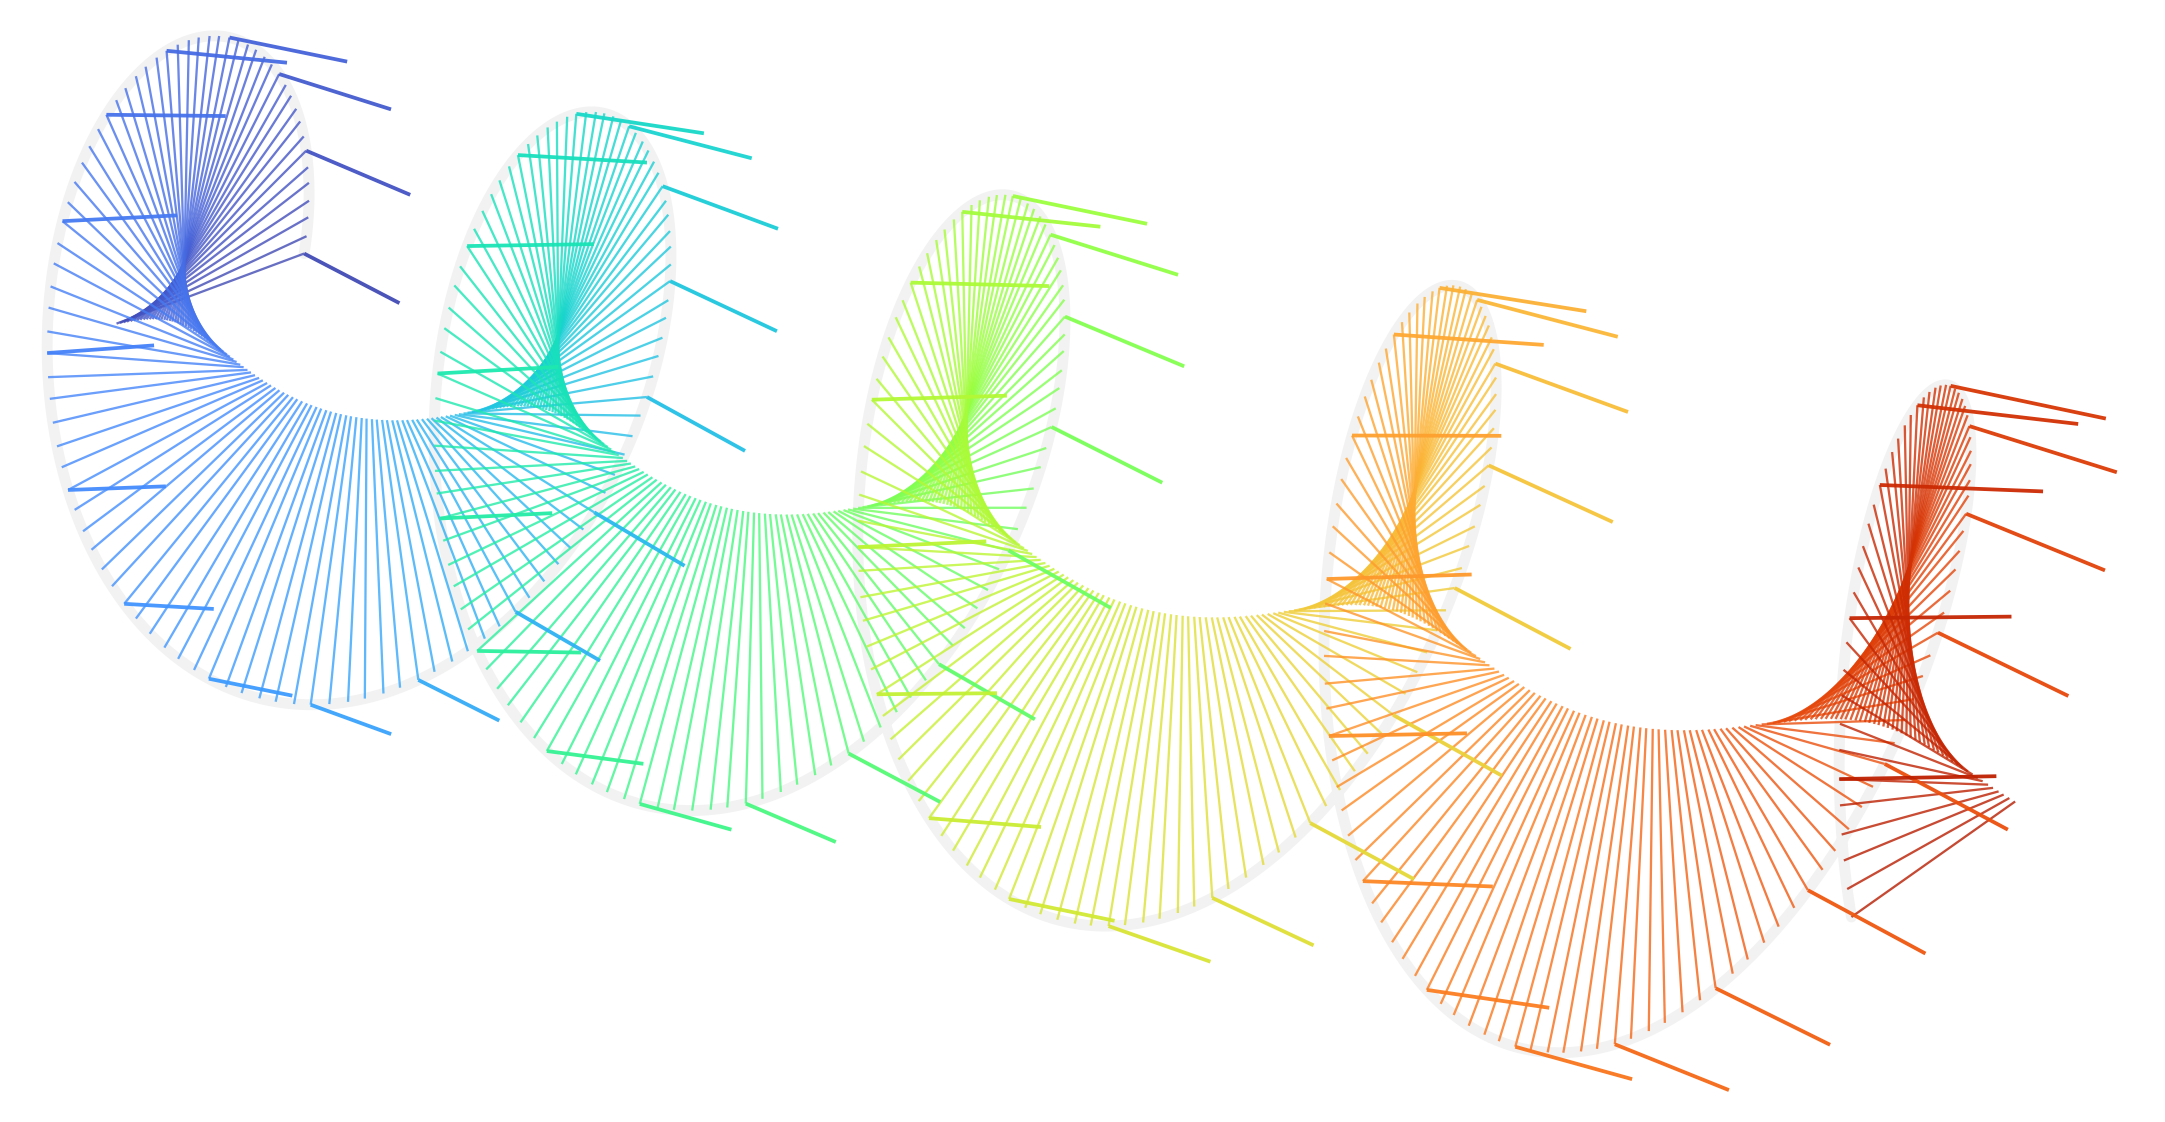
\includegraphics[width=1.0\textwidth]{figs/portada.png}\par
\vfill
{\small
$\displaystyle \vb{a}=\dot v\,\utau+\kappa v^{2}\,\un,\qquad
\oint_{\partial S}\vb{A}\cdot\dd\vb{r}=\int_{S}(\rot\vb{A})\cdot\dd\vb{S}$\par}
\vspace{9mm}
{\color{tenue!60}\rule{\textwidth}{0.4pt}}\par
\vspace{3mm}
{\small
\begin{tabular*}{\textwidth}{@{}l@{\extracolsep{\fill}}c@{\extracolsep{\fill}}r@{}}
{\color{cian}\scriptsize\textls[200]{\textsc{Autor}}} &
{\color{cian}\scriptsize\textls[200]{\textsc{Asignatura}}} &
{\color{cian}\scriptsize\textls[200]{\textsc{Apuntes formalizados}}}\\[0.6mm]
Daniel Martín Guerrero & Mecánica I (100810) & {\color{tenue}Salamanca, curso 2026/2027}\\
 & {\color{tenue}Teoría y seminario de problemas} & \\
\end{tabular*}}
\restoregeometry
\end{titlepage}

% =====================================================================
\setcounter{page}{2}
\tableofcontents
\clearpage

% =====================================================================
\section{La partícula en el espacio}
\label{sec:particula}
% =====================================================================

La mecánica newtoniana describe una partícula (punto material) mediante su
\emph{vector de posición} $\vb{r}(t)$ respecto de un origen $O$. La
\emph{cinemática} estudia $\vb{r}(t)$ y sus derivadas sin preguntar por las
causas del movimiento. Este tema reúne las herramientas geométricas que se
usarán en todo el curso: sistemas de coordenadas adaptados al problema
(\cref{sec:curvilineas}), geometría de curvas (\cref{sec:frenet}) y análisis
vectorial (\cref{sec:campos,sec:operadores,sec:integrales}).

\subsection{Trayectoria y órbita}

\begin{definicion}[Trayectoria, órbita]
Sea $I\subseteq\R$ un intervalo. Una \emph{trayectoria} es una aplicación
$\vb{r}\colon I\to\R^{3}$, $t\mapsto\vb{r}(t)$, de clase $\C^{2}(I)$. Su imagen
$\Gamma=\vb{r}(I)\subset\R^{3}$ es la \emph{órbita} (trayectoria geométrica).
Se definen la \emph{velocidad} y la \emph{aceleración}
\begin{equation}
  \vb{v}(t)\defeq\od{\vb{r}}{t}=\dot{\vb{r}},\qquad
  \vb{a}(t)\defeq\od{\vb{v}}{t}=\ddot{\vb{r}} .
  \label{eq:va-def}
\end{equation}
\end{definicion}

\begin{observacion}[Trayectoria frente a órbita]
Una misma órbita admite infinitas trayectorias: basta reparametrizar,
$\vb{r}=\vb{r}(\lambda)$ con $\lambda=\lambda(t)$. Por la regla de la cadena,
\begin{equation}
  \vb{v}=\od{\vb{r}}{\lambda}\,\od{\lambda}{t}.
  \label{eq:reparam}
\end{equation}
La \emph{órbita} contiene la información geométrica (curvatura, torsión;
\cref{sec:frenet}); la \emph{trayectoria} añade la ley horaria $s=s(t)$.
\end{observacion}

\subsection{Coordenadas, superficies y curvas coordenadas}

\begin{definicion}[Sistema de coordenadas]
\label{def:coordenadas}
Un \emph{sistema de coordenadas} en una región $D\subseteq\R^{3}$ es una
aplicación biyectiva de clase $\C^{1}$
\[
  (q^{1},q^{2},q^{3})\in U\subseteq\R^{3}\ \longmapsto\
  \vb{r}(q^{1},q^{2},q^{3})\in D,
  \qquad
  J\defeq\frac{\partial(x,y,z)}{\partial(q^{1},q^{2},q^{3})}\neq0,
\]
que asigna a cada punto $P$, de forma \emph{unívoca}, una terna
$(q^{1}_{P},q^{2}_{P},q^{3}_{P})$.
\begin{itemize}
  \item \emph{Superficies coordenadas}: $q^{i}=\text{const}$.
  \item \emph{Curvas coordenadas}: intersección de dos superficies
        coordenadas; a lo largo de la curva $q^{i}$ sólo varía $q^{i}$.
        Su vector tangente es $\partial\vb{r}/\partial q^{i}$.
  \item El sistema es \emph{ortogonal} si
        $\pd{\vb{r}}{q^{i}}\cdot\pd{\vb{r}}{q^{j}}=0$ para $i\neq j$ en todo
        punto.
\end{itemize}
\end{definicion}

\begin{ejemplo}[Cartesianas]
El punto de coordenadas $(1,2,3)$ es la intersección de los planos $x=1$,
$y=2$, $z=3$; las curvas coordenadas son rectas paralelas a los ejes y los
vectores tangentes, $(\ii,\jj,\kk)$, no dependen del punto.
\end{ejemplo}

\begin{clave}{Motivación}
En un campo de fuerzas centrales la aceleración depende sólo de la distancia
al origen, $r$: una única función en esféricas frente a tres en
cartesianas. Elegir coordenadas \emph{adaptadas a la simetría} reduce el
número de variables efectivas del problema.
\end{clave}

% ---------------------------------------------------------------------
\begin{figure}[t]
\centering
% ----------------------------- cilíndricas ---------------------------
\tdplotsetmaincoords{60}{118}
\begin{tikzpicture}[tdplot_main_coords,scale=1.22]
  \def\rP{2}\def\fP{78}\def\zP{2.1}
  % ejes
  \draw[eje] (0,0,0) -- (3.3,0,0) node[anchor=north east,peq,inner sep=1pt]{$x$};
  \draw[eje] (0,0,0) -- (0,3.1,0) node[anchor=north west,peq,inner sep=1pt]{$y$};
  \draw[eje] (0,0,0) -- (0,0,3.4) node[anchor=south,peq]{$z$};
  % cilindro rho = rP
  \draw[regla!80!tenue,line width=0.5pt] plot[domain=0:360,samples=90,smooth]
       ({\rP*cos(\x)},{\rP*sin(\x)},0);
  \draw[regla!80!tenue,line width=0.5pt] plot[domain=0:360,samples=90,smooth]
       ({\rP*cos(\x)},{\rP*sin(\x)},\zP);
  \draw[regla!80!tenue,line width=0.5pt] ({\rP*cos(28)},{\rP*sin(28)},0) -- ({\rP*cos(28)},{\rP*sin(28)},\zP);
  \draw[regla!80!tenue,line width=0.5pt] ({\rP*cos(208)},{\rP*sin(208)},0) -- ({\rP*cos(208)},{\rP*sin(208)},\zP);
  % proyección y ángulos
  \coordinate (O) at (0,0,0);
  \coordinate (Pp) at ({\rP*cos(\fP)},{\rP*sin(\fP)},0);
  \coordinate (P) at ({\rP*cos(\fP)},{\rP*sin(\fP)},\zP);
  \draw[aux] (O) -- (Pp) -- (P);
  \draw[aux] (0,0,\zP) -- (P);
  \draw[violeta,line width=0.6pt,->] plot[domain=0:\fP,samples=30]
       ({0.75*cos(\x)},{0.75*sin(\x)},0);
  \node[violeta,font=\small] at ({1.05*cos(\fP/2)},{1.05*sin(\fP/2)},0) {$\varphi$};
  \node[peq,anchor=north] at ($(O)!0.55!(Pp)$) {$\rho$};
  \node[peq,anchor=east] at (0,0,\zP) {$z$};
  % base local
  \draw[vec,cian] (P) -- ++({cos(\fP)},{sin(\fP)},0)
      node[anchor=north west,etiq,inner sep=1pt]{$\erho$};
  \draw[vec,violeta] (P) -- ++({-sin(\fP)},{cos(\fP)},0)
      node[anchor=west,etiq,inner sep=2pt]{$\ef$};
  \draw[vec,rosa] (P) -- ++(0,0,1)
      node[anchor=south,etiq,inner sep=1pt]{$\kk$};
  \node[punto] at (P) {};
  \node[etiq,anchor=south,inner sep=4pt] at (P) {$P$};
  \node[punto,fill=tenue,inner sep=0.9pt] at (Pp) {};
\end{tikzpicture}\hspace{4mm}%
% ----------------------------- esféricas -----------------------------
\tdplotsetmaincoords{60}{118}
\begin{tikzpicture}[tdplot_main_coords,scale=1.22]
  \def\rr{2.6}\def\tP{52}\def\fP{160}
  \pgfmathsetmacro{\px}{\rr*sin(\tP)*cos(\fP)}
  \pgfmathsetmacro{\py}{\rr*sin(\tP)*sin(\fP)}
  \pgfmathsetmacro{\pz}{\rr*cos(\tP)}
  \draw[eje] (0,0,0) -- (3.3,0,0) node[anchor=north east,peq,inner sep=1pt]{$x$};
  \draw[eje] (0,0,0) -- (0,3.1,0) node[anchor=north west,peq,inner sep=1pt]{$y$};
  \draw[eje] (0,0,0) -- (0,0,3.4) node[anchor=south,peq]{$z$};
  % silueta, ecuador y meridiano por P
  \draw[tdplot_screen_coords,regla!80!tenue,line width=0.5pt] (0,0) circle (\rr);
  \draw[regla!80!tenue,line width=0.5pt] plot[domain=0:360,samples=90,smooth]
       ({\rr*cos(\x)},{\rr*sin(\x)},0);
  \draw[regla!80!tenue,line width=0.5pt] plot[domain=0:180,samples=60,smooth]
       ({\rr*sin(\x)*cos(\fP)},{\rr*sin(\x)*sin(\fP)},{\rr*cos(\x)});
  \coordinate (O) at (0,0,0);
  \coordinate (P) at (\px,\py,\pz);
  \coordinate (Pp) at (\px,\py,0);
  \draw[texto,line width=0.6pt] (O) -- (P);
  \draw[aux] (O) -- (Pp) -- (P);
  % ángulos
  \draw[violeta,line width=0.6pt,->] plot[domain=0:\fP,samples=30]
       ({0.7*cos(\x)},{0.7*sin(\x)},0);
  \node[violeta,font=\small] at ({1.0*cos(\fP/2)},{1.0*sin(\fP/2)},0) {$\varphi$};
  \draw[cian,line width=0.6pt,->] plot[domain=0:\tP,samples=30]
       ({1.1*sin(\x)*cos(\fP)},{1.1*sin(\x)*sin(\fP)},{1.1*cos(\x)});
  \node[cian,font=\small] at ({1.42*sin(\tP/2)*cos(\fP)},{1.42*sin(\tP/2)*sin(\fP)},{1.42*cos(\tP/2)}) {$\theta$};
  \node[peq,anchor=north west,inner sep=1.5pt] at ($(O)!0.6!(P)$) {$r$};
  % base local
  \draw[vec,cian] (P) -- ++({sin(\tP)*cos(\fP)},{sin(\tP)*sin(\fP)},{cos(\tP)})
      node[anchor=south west,etiq,inner sep=1pt]{$\er$};
  \draw[vec,rosa] (P) -- ++({cos(\tP)*cos(\fP)},{cos(\tP)*sin(\fP)},{-sin(\tP)})
      node[anchor=north west,etiq,inner sep=1pt]{$\et$};
  \draw[vec,violeta] (P) -- ++({-sin(\fP)},{cos(\fP)},0)
      node[anchor=south east,etiq,inner sep=1pt]{$\ef$};
  \node[punto] at (P) {};
  \node[etiq,anchor=south,inner sep=4pt] at (P) {$P$};
\end{tikzpicture}
\caption{Coordenadas cilíndricas $(\rho,\varphi,z)$ (izquierda) y esféricas
$(r,\theta,\varphi)$ (derecha). En cada punto $P$ la base local está formada
por los vectores unitarios tangentes a las tres curvas coordenadas que pasan
por $P$; cambia de un punto a otro.}
\label{fig:cil-esf}
\end{figure}
% ---------------------------------------------------------------------

\subsection{Producto mixto y símbolo de Levi-Civita}

\begin{definicion}[Símbolo de Levi-Civita]
Para $i,j,k\in\{1,2,3\}$,
\begin{equation}
  \varepsilon_{ijk}=
  \begin{cases}
    +1, & (i,j,k)\ \text{permutación par de }(1,2,3),\\
    -1, & (i,j,k)\ \text{permutación impar de }(1,2,3),\\
    \ \ 0, & \text{si dos índices coinciden},
  \end{cases}
  \qquad \varepsilon_{123}=+1 .
\end{equation}
Se adopta el \emph{convenio de suma de Einstein}: los índices repetidos se suman
de $1$ a $3$.
\end{definicion}

Con él, $(\vb{b}\times\vb{c})_{i}=\varepsilon_{ijk}b_{j}c_{k}$ y el producto
mixto es un determinante:
\begin{equation}
  \vb{a}\cdot(\vb{b}\times\vb{c})=\varepsilon_{ijk}\,a_{i}b_{j}c_{k}
  =\det\begin{pmatrix}a_{1}&a_{2}&a_{3}\\ b_{1}&b_{2}&b_{3}\\ c_{1}&c_{2}&c_{3}\end{pmatrix},
  \qquad
  V_{\text{paralelepípedo}}=\abs{\vb{a}\cdot(\vb{b}\times\vb{c})}.
  \label{eq:mixto}
\end{equation}

\begin{lema}[Contracción $\varepsilon$--$\delta$]
\label{lem:epsdelta}
$\varepsilon_{ijk}\,\varepsilon_{imn}=\delta_{jm}\delta_{kn}-\delta_{jn}\delta_{km}$.
\end{lema}

\begin{proof}
Ambos miembros son nulos si $j=k$ o $m=n$. Si $j\neq k$, el único $i$ que
contribuye es el tercer índice, y $\varepsilon_{ijk}\varepsilon_{imn}\neq0$
sólo si $\{m,n\}=\{j,k\}$: vale $+1$ si $(m,n)=(j,k)$ y $-1$ si
$(m,n)=(k,j)$, exactamente lo que da el miembro derecho.
\end{proof}

\begin{corolario}[Doble producto vectorial]
\label{cor:bac}
$\vb{a}\times(\vb{b}\times\vb{c})=\vb{b}\,(\vb{a}\cdot\vb{c})-\vb{c}\,(\vb{a}\cdot\vb{b})$.
\end{corolario}

\begin{proof}
Por el \cref{lem:epsdelta}, con $\varepsilon_{ijk}=\varepsilon_{kij}$,
\[
[\vb{a}\times(\vb{b}\times\vb{c})]_{i}
=\varepsilon_{kij}\varepsilon_{kmn}\,a_{j}b_{m}c_{n}
=(\delta_{im}\delta_{jn}-\delta_{in}\delta_{jm})\,a_{j}b_{m}c_{n}
=b_{i}(\vb{a}\cdot\vb{c})-c_{i}(\vb{a}\cdot\vb{b}).\qedhere
\]
\end{proof}

% =====================================================================
\section{Coordenadas curvilíneas ortogonales}
\label{sec:curvilineas}
% =====================================================================

Todo el problema de escribir magnitudes mecánicas en un sistema de
coordenadas se reduce a dos datos: \emph{cuánto} se desplaza el punto al
variar cada coordenada (los factores de escala $h_{i}$) y \emph{cómo gira}
la base local de un punto a otro (las derivadas $\dd\uv{e}_{i}$).

\subsection{Factores de escala y base local}

\begin{definicion}[Factores de escala, base local]
\label{def:escala}
Sea $\vb{r}=\vb{r}(q^{1},q^{2},q^{3})$ un sistema de coordenadas
(\cref{def:coordenadas}). Se definen los \emph{factores (parámetros) de
escala} y los \emph{vectores unitarios} de la base local
\begin{equation}
  h_{i}\defeq\norm{\pd{\vb{r}}{q^{i}}},\qquad
  \uv{e}_{i}\defeq\frac{1}{h_{i}}\pd{\vb{r}}{q^{i}},\qquad i=1,2,3
  \quad(\text{sin suma}).
  \label{eq:escala}
\end{equation}
El sistema es \emph{ortogonal} si $\uv{e}_{i}\cdot\uv{e}_{j}=\delta_{ij}$, y
lo supondremos además \emph{dextrógiro}: $\uv{e}_{1}\times\uv{e}_{2}=\uv{e}_{3}$.
\end{definicion}

\begin{proposicion}[Desplazamiento y métrica]
\label{prop:metrica}
En un sistema ortogonal,
\begin{equation}
  \dd\vb{r}=\sum_{i=1}^{3}h_{i}\,\dd q^{i}\,\uv{e}_{i},
  \qquad
  \dd s^{2}\defeq\dd\vb{r}\cdot\dd\vb{r}
  =h_{1}^{2}(\dd q^{1})^{2}+h_{2}^{2}(\dd q^{2})^{2}+h_{3}^{2}(\dd q^{3})^{2}.
  \label{eq:metrica}
\end{equation}
\end{proposicion}

\begin{proof}
Por la regla de la cadena,
$\dd\vb{r}=\sum_{i}\pd{\vb{r}}{q^{i}}\dd q^{i}=\sum_{i}h_{i}\dd q^{i}\uv{e}_{i}$
por \eqref{eq:escala}. Al multiplicar escalarmente, los términos cruzados se
anulan por ortogonalidad.
\end{proof}

\begin{clave}{Dos maneras de obtener los $h_{i}$}
\begin{enumerate}[leftmargin=1.4em]
  \item \emph{Por definición}: derivar $\vb{r}$ (en cartesianas) respecto de
        cada $q^{i}$ y tomar el módulo, \eqref{eq:escala}.
  \item \emph{Leyéndolos en $\dd s^{2}$}: escribir $\dd x,\dd y,\dd z$ en
        función de $\dd q^{i}$, desarrollar $\dd x^{2}+\dd y^{2}+\dd z^{2}$ y
        comprobar que no hay términos cruzados $\dd q^{i}\dd q^{j}$ (ortogonalidad);
        los coeficientes de $(\dd q^{i})^{2}$ son $h_{i}^{2}$.
\end{enumerate}
\end{clave}

\begin{observacion}[El vector de posición]
En general $\vb{r}\neq\sum_{i}q^{i}\uv{e}_{i}$: en esféricas
$\vb{r}=r\,\er$ (no aparecen $\theta$ ni $\varphi$) y en cilíndricas
$\vb{r}=\rho\,\erho+z\,\kk$. Lo que sí es universal es la forma
\eqref{eq:metrica} del \emph{desplazamiento} $\dd\vb{r}$.
\end{observacion}

\subsection{Elementos de línea, superficie y volumen}

\begin{proposicion}[Elementos diferenciales]
\label{prop:elementos}
En un sistema ortogonal dextrógiro, con $(i,j,k)$ permutación cíclica de
$(1,2,3)$:
\begin{align}
  \dd\vb{l}_{i}&=h_{i}\,\dd q^{i}\,\uv{e}_{i},
  &&\text{(línea)}\label{eq:dl}\\
  \dd\vb{S}_{i}&=\dd\vb{l}_{j}\times\dd\vb{l}_{k}=h_{j}h_{k}\,\dd q^{j}\dd q^{k}\,\uv{e}_{i},
  &&\text{(superficie)}\label{eq:dS}\\
  \dd V&=(\dd\vb{l}_{1}\times\dd\vb{l}_{2})\cdot\dd\vb{l}_{3}=h_{1}h_{2}h_{3}\,\dd q^{1}\dd q^{2}\dd q^{3}.
  &&\text{(volumen)}\label{eq:dV}
\end{align}
Además, el jacobiano del cambio de variables es
$J=\dfrac{\partial(x,y,z)}{\partial(q^{1},q^{2},q^{3})}=h_{1}h_{2}h_{3}$.
\end{proposicion}

\begin{proof}
\eqref{eq:dS} y \eqref{eq:dV} son productos vectoriales y mixtos de
\eqref{eq:dl}, con $\uv{e}_{j}\times\uv{e}_{k}=\uv{e}_{i}$. Para $J$: sus
columnas son $\partial\vb{r}/\partial q^{i}=h_{i}\uv{e}_{i}$, luego, por
\eqref{eq:mixto},
$J=h_{1}h_{2}h_{3}\,\uv{e}_{1}\cdot(\uv{e}_{2}\times\uv{e}_{3})=h_{1}h_{2}h_{3}$.
\end{proof}

% ---------------------------------------------------------------------
\begin{figure}[ht]
\centering
\begin{tikzpicture}[scale=1.15]
  \def\W{3.2}\def\H{2.0}\def\dx{1.5}\def\dy{0.95}
  % caras q^1 (izquierda) y q^1+dq^1 (derecha)
  \fill[cian,opacity=0.10] (0,0) -- (\dx,\dy) -- (\dx,\H+\dy) -- (0,\H) -- cycle;
  \fill[cian,opacity=0.22] (\W,0) -- (\W+\dx,\dy) -- (\W+\dx,\H+\dy) -- (\W,\H) -- cycle;
  % aristas ocultas
  \draw[aux] (0,0) -- (\dx,\dy) -- (\W+\dx,\dy);
  \draw[aux] (\dx,\dy) -- (\dx,\H+\dy);
  % aristas visibles
  \draw[texto!75,line width=0.55pt] (0,0) rectangle (\W,\H);
  \draw[texto!75,line width=0.55pt] (\W,0) -- (\W+\dx,\dy) -- (\W+\dx,\H+\dy) -- (\W,\H);
  \draw[texto!75,line width=0.55pt] (0,\H) -- (\dx,\H+\dy) -- (\W+\dx,\H+\dy);
  % cotas
  \node[etiq,anchor=north,inner sep=4pt] at (\W/2,0) {$h_{1}\dd q^{1}$};
  \node[etiq,anchor=north west,inner sep=2pt] at (\W+\dx/2,\dy/2) {$h_{2}\dd q^{2}$};
  \node[etiq,anchor=west,inner sep=3pt] at (\W+\dx,\H+\dy-0.35) {$h_{3}\dd q^{3}$};
  % vértice de referencia
  \node[punto,fill=tenue,inner sep=1pt] at (0,0) {};
  \node[peq,anchor=north east,inner sep=2pt] at (0,0) {$(q^{1},q^{2},q^{3})$};
  % normales salientes
  \draw[vec,cian] (\W+\dx/2,\H/2+\dy/2) -- ++(1.2,0)
     node[anchor=west,etiq,inner sep=2pt]{$\uv{e}_{1}$};
  \draw[vec,cian!60!tenue] (\dx/2,\H/2+\dy/2) -- ++(-1.2,0)
     node[anchor=east,etiq,inner sep=2pt]{$-\uv{e}_{1}$};
  \node[cian,font=\footnotesize,anchor=south,inner sep=3pt] at (\W+\dx/2,\H+\dy) {$q^{1}+\dd q^{1}$};
  \node[cian!60!tenue,font=\footnotesize,anchor=south,inner sep=3pt] at (\dx/2,\H+\dy) {$q^{1}$};
\end{tikzpicture}
\caption{Paralelepípedo elemental de un sistema ortogonal: aristas
$h_{i}\dd q^{i}$ y volumen $\dd V=h_{1}h_{2}h_{3}\dd q^{1}\dd q^{2}\dd q^{3}$.
Las caras sombreadas, $q^{1}$ y $q^{1}+\dd q^{1}$, con normales salientes
$\mp\uv{e}_{1}$, son las que intervienen en el cálculo de la divergencia
(\cref{sec:div-curv}).}
\label{fig:caja}
\end{figure}
% ---------------------------------------------------------------------

\subsection{Coordenadas cartesianas y cilíndricas}

\paragraph{Cartesianas.} $(q^{1},q^{2},q^{3})=(x,y,z)$,
$\vb{r}=x\ii+y\jj+z\kk$, base fija ($\dd\ii=\dd\jj=\dd\kk=\vb{0}$) y
$h_{x}=h_{y}=h_{z}=1$:
\begin{equation}
  \dd s^{2}=\dd x^{2}+\dd y^{2}+\dd z^{2},\quad
  \dd\vb{S}=(\dd y\,\dd z\,\ii,\ \dd z\,\dd x\,\jj,\ \dd x\,\dd y\,\kk),\quad
  \dd V=\dd x\,\dd y\,\dd z .
\end{equation}

\begin{definicion}[Coordenadas cilíndricas]
$(q^{1},q^{2},q^{3})=(\rho,\varphi,z)$ con $\rho\ge0$, $\varphi\in[0,2\pi)$:
\begin{equation}
  x=\rho\cos\varphi,\quad y=\rho\sin\varphi,\quad z=z
  \qquad\Longleftrightarrow\qquad
  \rho=\sqrt{x^{2}+y^{2}},\quad \varphi=\arctan(y/x).
  \label{eq:cil}
\end{equation}
Superficies coordenadas: cilindros ($\rho=\text{const}$), semiplanos
($\varphi=\text{const}$) y planos ($z=\text{const}$).
\end{definicion}

Aplicando \eqref{eq:escala} a $\vb{r}=\rho\cos\varphi\,\ii+\rho\sin\varphi\,\jj+z\,\kk$:
\begin{equation}
  \pd{\vb{r}}{\rho}=\cos\varphi\,\ii+\sin\varphi\,\jj,\qquad
  \pd{\vb{r}}{\varphi}=\rho\,(-\sin\varphi\,\ii+\cos\varphi\,\jj),\qquad
  \pd{\vb{r}}{z}=\kk,
\end{equation}
de donde
\begin{equation}
  \resultado{
  \begin{gathered}
  h_{\rho}=1,\qquad h_{\varphi}=\rho,\qquad h_{z}=1,\\
  \erho=\cos\varphi\,\ii+\sin\varphi\,\jj,\quad
  \ef=-\sin\varphi\,\ii+\cos\varphi\,\jj,\quad \uv{e}_{z}=\kk .
  \end{gathered}}
  \label{eq:cil-base}
\end{equation}
La base es ortonormal y dextrógira ($\erho\times\ef=\kk$). Además
$\vb{r}=\rho\,\erho+z\,\kk$ y, por \cref{prop:metrica,prop:elementos},
\begin{gather}
  \dd\vb{r}=\dd\rho\,\erho+\rho\,\dd\varphi\,\ef+\dd z\,\kk,\qquad
  \dd s^{2}=\dd\rho^{2}+\rho^{2}\dd\varphi^{2}+\dd z^{2},\\
  \dd\vb{S}_{\rho}=\rho\,\dd\varphi\,\dd z\,\erho,\quad
  \dd\vb{S}_{\varphi}=\dd z\,\dd\rho\,\ef,\quad
  \dd\vb{S}_{z}=\rho\,\dd\rho\,\dd\varphi\,\kk,\qquad
  \dd V=\rho\,\dd\rho\,\dd\varphi\,\dd z .
  \label{eq:cil-elem}
\end{gather}

\subsection{Coordenadas esféricas}

\begin{definicion}[Coordenadas esféricas]
$(q^{1},q^{2},q^{3})=(r,\theta,\varphi)$ con $r\ge0$, $\theta\in[0,\pi]$,
$\varphi\in[0,2\pi)$:
\begin{equation}
  \begin{aligned}
  x&=r\sin\theta\cos\varphi,\\ y&=r\sin\theta\sin\varphi,\\ z&=r\cos\theta,
  \end{aligned}
  \qquad\Longleftrightarrow\qquad
  \begin{aligned}
  r&=\sqrt{x^{2}+y^{2}+z^{2}},\\ \theta&=\arccos(z/r),\\ \varphi&=\arctan(y/x).
  \end{aligned}
  \label{eq:esf}
\end{equation}
Superficies coordenadas: esferas ($r$), conos de vértice $O$ ($\theta$) y
semiplanos de borde el eje $z$ ($\varphi$).
\end{definicion}

Derivando $\vb{r}=r\sin\theta\cos\varphi\,\ii+r\sin\theta\sin\varphi\,\jj+r\cos\theta\,\kk$:
\begin{equation}
  \pd{\vb{r}}{r}=\er,\qquad
  \pd{\vb{r}}{\theta}=r\,\et,\qquad
  \pd{\vb{r}}{\varphi}=r\sin\theta\,\ef,
\end{equation}
con
\begin{equation}
  \resultado{
  \begin{aligned}
  \er&=\sin\theta\cos\varphi\,\ii+\sin\theta\sin\varphi\,\jj+\cos\theta\,\kk,\\
  \et&=\cos\theta\cos\varphi\,\ii+\cos\theta\sin\varphi\,\jj-\sin\theta\,\kk,\\
  \ef&=-\sin\varphi\,\ii+\cos\varphi\,\jj,
  \end{aligned}
  \qquad
  \begin{aligned}
  h_{r}&=1,\\ h_{\theta}&=r,\\ h_{\varphi}&=r\sin\theta .
  \end{aligned}}
  \label{eq:esf-base}
\end{equation}
La base es ortonormal y dextrógira ($\er\times\et=\ef$), $\vb{r}=r\,\er$, y
\begin{gather}
  \dd\vb{r}=\dd r\,\er+r\,\dd\theta\,\et+r\sin\theta\,\dd\varphi\,\ef,\qquad
  \dd s^{2}=\dd r^{2}+r^{2}\dd\theta^{2}+r^{2}\sin^{2}\theta\,\dd\varphi^{2},\\
  \dd\vb{S}_{r}=r^{2}\sin\theta\,\dd\theta\,\dd\varphi\,\er,\quad
  \dd\vb{S}_{\theta}=r\sin\theta\,\dd\varphi\,\dd r\,\et,\quad
  \dd\vb{S}_{\varphi}=r\,\dd r\,\dd\theta\,\ef,\\
  \dd V=r^{2}\sin\theta\,\dd r\,\dd\theta\,\dd\varphi .
  \label{eq:esf-elem}
\end{gather}

\subsection{La base móvil y sus derivadas}

A diferencia de $(\ii,\jj,\kk)$, la base curvilínea depende del punto. Sus
diferenciales se obtienen derivando \eqref{eq:cil-base} y \eqref{eq:esf-base}.

\begin{proposicion}[Diferenciales de la base]
\label{prop:dbase}
\begin{align}
  &\text{Cilíndricas:} &
  \dd\erho&=\dd\varphi\,\ef,\qquad \dd\ef=-\dd\varphi\,\erho,\qquad \dd\kk=\vb{0};
  \label{eq:dcil}\\[1mm]
  &\text{Esféricas:} &
  \dd\er&=\dd\theta\,\et+\sin\theta\,\dd\varphi\,\ef,\notag\\
  && \dd\et&=-\dd\theta\,\er+\cos\theta\,\dd\varphi\,\ef,\label{eq:desf}\\
  && \dd\ef&=-\dd\varphi\,(\sin\theta\,\er+\cos\theta\,\et).\notag
\end{align}
\end{proposicion}

\begin{proof}
Cilíndricas: $\dd\erho=\dd\varphi(-\sin\varphi\,\ii+\cos\varphi\,\jj)=\dd\varphi\,\ef$
y $\dd\ef=-\dd\varphi(\cos\varphi\,\ii+\sin\varphi\,\jj)=-\dd\varphi\,\erho$.
Esféricas: $\partial_{\theta}\er=\et$ y
$\partial_{\varphi}\er=\sin\theta(-\sin\varphi\,\ii+\cos\varphi\,\jj)=\sin\theta\,\ef$;
$\partial_{\theta}\et=-\er$ y $\partial_{\varphi}\et=\cos\theta\,\ef$;
finalmente $\dd\ef=-\dd\varphi(\cos\varphi\,\ii+\sin\varphi\,\jj)$ y
$\cos\varphi\,\ii+\sin\varphi\,\jj=\sin\theta\,\er+\cos\theta\,\et$
(proyección horizontal de \eqref{eq:esf-base}).
\end{proof}

\begin{clave}[violeta]{Lectura compacta: la base gira}
Las fórmulas anteriores son $\dd\uv{e}_{i}=\dd\vb{\Omega}\times\uv{e}_{i}$ con
el «ángulo de giro» de la base
\begin{equation}
  \dd\vb{\Omega}_{\text{cil}}=\dd\varphi\,\kk,\qquad
  \dd\vb{\Omega}_{\text{esf}}=\dd\varphi\,\kk+\dd\theta\,\ef,
  \qquad \kk=\cos\theta\,\er-\sin\theta\,\et .
  \label{eq:omega-base}
\end{equation}
Por ejemplo, $\dd\vb{\Omega}_{\text{esf}}\times\er
=\dd\varphi\sin\theta\,\ef+\dd\theta\,\et$. Basta recordar
$\dd\vb{\Omega}$ y la regla del producto vectorial.
\end{clave}

\begin{table}[ht]
\centering
\caption{Datos esenciales de los tres sistemas ortogonales usuales.}
\label{tab:sistemas}
\small
\begin{tabular}{@{}l c c c c@{}}
\toprule
\color{cian} Sistema & \color{cian} $(q^{1},q^{2},q^{3})$ & \color{cian} $(h_{1},h_{2},h_{3})$
 & \color{cian} $\vb{r}$ & \color{cian} $\dd V$\\
\midrule
Cartesianas & $(x,y,z)$ & $(1,1,1)$ & $x\ii+y\jj+z\kk$ & $\dd x\,\dd y\,\dd z$\\
Cilíndricas & $(\rho,\varphi,z)$ & $(1,\rho,1)$ & $\rho\,\erho+z\,\kk$ & $\rho\,\dd\rho\,\dd\varphi\,\dd z$\\
Esféricas & $(r,\theta,\varphi)$ & $(1,r,r\sin\theta)$ & $r\,\er$ & $r^{2}\sin\theta\,\dd r\,\dd\theta\,\dd\varphi$\\
\bottomrule
\end{tabular}
\end{table}

% =====================================================================
\section{Cinemática de la partícula}
\label{sec:cinematica}
% =====================================================================

\subsection{Derivada de un vector y vector tangente}

\begin{definicion}[Vector tangente]
Sea $\vb{r}=\vb{r}(\lambda)$, $\lambda\in I$, una curva de clase $\C^{1}$. El
\emph{vector tangente} en $\lambda$ es
\begin{equation}
  \vb{t}(\lambda)\defeq\lim_{\Delta\lambda\to0}\frac{\vb{r}(\lambda+\Delta\lambda)-\vb{r}(\lambda)}{\Delta\lambda}
  =\od{\vb{r}}{\lambda}.
\end{equation}
En la base fija, la derivada actúa componente a componente:
$\od{\vb{r}}{\lambda}=\od{x}{\lambda}\ii+\od{y}{\lambda}\jj+\od{z}{\lambda}\kk$.
\end{definicion}

Con $\lambda=t$ el vector tangente es la velocidad; con $\lambda=s$ (longitud
de arco, \cref{sec:frenet}) es unitario, $\utau=\dd\vb{r}/\dd s=\vb{v}/v$.

\begin{clave}{Regla operativa}
En una base \emph{móvil} la derivada actúa también sobre los vectores de la
base: si $\vb{A}=\sum_{i}A_{i}\uv{e}_{i}$,
\begin{equation}
  \od{\vb{A}}{t}=\sum_{i}\dot A_{i}\,\uv{e}_{i}+\sum_{i}A_{i}\,\duv{e}{i},
  \qquad \duv{e}{i}=\vb{\Omega}\times\uv{e}_{i},\quad
  \vb{\Omega}\,\dd t=\dd\vb{\Omega}\ \text{de \eqref{eq:omega-base}}.
  \label{eq:derivada-movil}
\end{equation}
\end{clave}

\subsection{Velocidad y aceleración en las tres bases}

\begin{proposicion}[Velocidad y aceleración]
\label{prop:va}
Para una partícula de trayectoria $\vb{r}(t)$:
\begin{enumerate}[label=\textcolor{cian}{(\roman*)},leftmargin=2em]
  \item \emph{Cartesianas}:
  \begin{equation}
    \vb{v}=\dot x\,\ii+\dot y\,\jj+\dot z\,\kk,\qquad
    \vb{a}=\ddot x\,\ii+\ddot y\,\jj+\ddot z\,\kk .
  \end{equation}
  \item \emph{Cilíndricas}:
  \begin{equation}
    \vb{v}=\dot\rho\,\erho+\rho\dot\varphi\,\ef+\dot z\,\kk,\qquad
    \vb{a}=(\ddot\rho-\rho\dot\varphi^{2})\,\erho
    +(\rho\ddot\varphi+2\dot\rho\dot\varphi)\,\ef+\ddot z\,\kk .
    \label{eq:va-cil}
  \end{equation}
  \item \emph{Esféricas}:
  \begin{equation}
    \begin{aligned}
    \vb{v}&=\dot r\,\er+r\dot\theta\,\et+r\sin\theta\,\dot\varphi\,\ef,\\
    \vb{a}&=\bigl(\ddot r-r\dot\theta^{2}-r\sin^{2}\!\theta\,\dot\varphi^{2}\bigr)\er
     +\bigl(r\ddot\theta+2\dot r\dot\theta-r\sin\theta\cos\theta\,\dot\varphi^{2}\bigr)\et\\
     &\quad+\bigl(r\sin\theta\,\ddot\varphi+2\dot r\dot\varphi\sin\theta+2r\dot\theta\dot\varphi\cos\theta\bigr)\ef .
    \end{aligned}
    \label{eq:va-esf}
  \end{equation}
\end{enumerate}
\end{proposicion}

La demostración es el \cref{prob:1} del seminario
(\cref{sec:seminario}); conviene rehacerla hasta que sea automática.

\begin{observacion}[Forma «de momento angular»]
Las componentes azimutales se compactan como derivadas totales:
\begin{equation}
  a_{\varphi}^{\text{cil}}=\frac{1}{\rho}\od{}{t}\bigl(\rho^{2}\dot\varphi\bigr),
  \qquad
  a_{\theta}^{\text{esf}}=\frac{1}{r}\od{}{t}\bigl(r^{2}\dot\theta\bigr)-r\sin\theta\cos\theta\,\dot\varphi^{2},
  \qquad
  a_{\varphi}^{\text{esf}}=\frac{1}{r\sin\theta}\od{}{t}\bigl(r^{2}\sin^{2}\!\theta\,\dot\varphi\bigr).
\end{equation}
Si $a_{\varphi}=0$ (fuerza central), $\rho^{2}\dot\varphi$ se conserva: es la
semilla de la ley de las áreas (Tema 4).
\end{observacion}

\begin{observacion}[Interpretación de cada término]
En \eqref{eq:va-cil}: $-\rho\dot\varphi^{2}$ es la aceleración
\emph{centrípeta}, $\rho\ddot\varphi$ la \emph{angular} y
$2\dot\rho\dot\varphi$ la de \emph{Coriolis}, que aparece porque al moverse
radialmente cambia el radio de giro.
\end{observacion}

% =====================================================================
\section{Curvas en el espacio: triedro intrínseco}
\label{sec:frenet}
% =====================================================================

La base adaptada a la \emph{órbita} (no a unas coordenadas) es el triedro de
Frenet: tangente, normal y binormal. En ella la aceleración se separa en una
parte que cambia el módulo de $\vb{v}$ y otra que cambia su dirección.

\subsection{Longitud de arco y triedro de Frenet}

\begin{definicion}[Longitud de arco]
\label{def:arco}
Para una curva regular $\vb{r}(t)$ ($\dot{\vb{r}}\neq\vb{0}$), la
\emph{longitud de arco} desde $t_{0}$ es
\begin{equation}
  s(t)=\int_{t_{0}}^{t}\norm{\dot{\vb{r}}(t')}\dd t'
      =\int_{t_{0}}^{t}\sqrt{\dot x^{2}+\dot y^{2}+\dot z^{2}}\,\dd t',
  \qquad \od{s}{t}=\norm{\vb{v}}=v,\qquad \dd s^{2}=\dd\vb{r}\cdot\dd\vb{r}.
  \label{eq:arco}
\end{equation}
\end{definicion}

\begin{observacion}[La longitud como funcional]
Un \emph{funcional} asigna un número a cada función. La longitud de una curva
lo es: la variable es la curva entera.
\begin{enumerate}
  \item \emph{Gráfica $y=y(x)$ en el plano}:
  \[
    L[y]=\int_{a}^{b}\sqrt{1+y'(x)^{2}}\;\dd x,
    \qquad\text{de la forma } \int_{a}^{b}F(x,y,y')\,\dd x \text{ con } F=\sqrt{1+y'^{2}}.
  \]
  \item \emph{Curva paramétrica}:
  \[
    L[\vb{r}]=\int_{t_{0}}^{t_{1}}\norm{\dot{\vb{r}}(t)}\,\dd t
    =\int_{t_{0}}^{t_{1}}\sqrt{\dot x^{2}+\dot y^{2}+\dot z^{2}}\;\dd t .
  \]
  \item \emph{En coordenadas curvilíneas}, por \eqref{eq:metrica}; por ejemplo, sobre la esfera $r=R$:
  \[
    L[\vb{q}]=\int_{t_{0}}^{t_{1}}\sqrt{h_{1}^{2}(\dot q^{1})^{2}+h_{2}^{2}(\dot q^{2})^{2}+h_{3}^{2}(\dot q^{3})^{2}}\;\dd t,
    \qquad
    L[\theta,\varphi]=R\int_{t_{0}}^{t_{1}}\sqrt{\dot\theta^{2}+\sin^{2}\theta\,\dot\varphi^{2}}\;\dd t .
  \]
\end{enumerate}
\emph{Función frente a funcional}: $s(t)$ en \eqref{eq:arco} es una
\emph{función} de $t$ (la curva está fija); $L[\vb{r}]$ es un \emph{funcional}
(cambia la curva y cambia el número). Además $L$ no depende de la
parametrización: con $t=t(\lambda)$,
$\norm{\dd\vb{r}/\dd t}\,\dd t=\norm{\dd\vb{r}/\dd\lambda}\,\dd\lambda$, así que es una
propiedad de la \emph{órbita}, no de la trayectoria.
\end{observacion}

\begin{definicion}[Triedro de Frenet, curvatura, torsión]
\label{def:frenet}
Parametrizando por $s$ y suponiendo $\dd\utau/\dd s\neq\vb{0}$:
\begin{equation}
  \utau\defeq\od{\vb{r}}{s},\qquad
  \kappa\defeq\norm{\od{\utau}{s}},\qquad
  \un\defeq\frac{1}{\kappa}\od{\utau}{s},\qquad
  \ub\defeq\utau\times\un .
  \label{eq:triedro}
\end{equation}
$\kappa$ es la \emph{curvatura} y $\rho_{c}=1/\kappa$ el \emph{radio de
curvatura}. La \emph{torsión} $\tors$ se define en \eqref{eq:frenet} por
$\dd\ub/\dd s=-\tors\,\un$.
\end{definicion}

\begin{lema}[Derivada de un vector unitario]
\label{lem:unitario}
Si $\norm{\uv{a}(s)}=1$ para todo $s$, entonces $\uv{a}\perp\dd\uv{a}/\dd s$.
\end{lema}

\begin{proof}
$0=\od{}{s}(1)=\od{}{s}(\uv{a}\cdot\uv{a})=2\,\uv{a}\cdot\od{\uv{a}}{s}$.
\end{proof}

En particular $\un\perp\utau$, de modo que $(\utau,\un,\ub)$ es una base
ortonormal dextrógira en cada punto de la curva.

\subsection{Fórmulas de Frenet--Serret}

\begin{teorema}[Frenet--Serret]
\label{teo:frenet}
Existe una función $\tors(s)$, la \emph{torsión}, tal que
\begin{equation}
  \resultado{\od{\utau}{s}=\kappa\,\un,\qquad
  \od{\un}{s}=-\kappa\,\utau+\tors\,\ub,\qquad
  \od{\ub}{s}=-\tors\,\un}
  \label{eq:frenet}
\end{equation}
o, en forma matricial,
\begin{equation}
  \od{}{s}\begin{pmatrix}\utau\\ \un\\ \ub\end{pmatrix}
  =\begin{pmatrix}0&\kappa&0\\ -\kappa&0&\tors\\ 0&-\tors&0\end{pmatrix}
  \begin{pmatrix}\utau\\ \un\\ \ub\end{pmatrix}.
\end{equation}
\end{teorema}

\begin{proof}
\begin{enumerate}
  \item \emph{Primera}: es la definición \eqref{eq:triedro}.
  \item \emph{Tercera}. Por el \cref{lem:unitario}, $\ub'\perp\ub$. Además
  $\ub'=(\utau\times\un)'=\utau'\times\un+\utau\times\un'
  =\kappa\,\un\times\un+\utau\times\un'=\utau\times\un'$, que es
  $\perp\utau$. Ortogonal a $\ub$ y a $\utau$, $\ub'$ es paralelo a $\un$:
  $\ub'=-\tors\,\un$ define $\tors$.
  \item \emph{Segunda}. Se descompone $\un'$ en la base:
  $\utau\cdot\un'=(\utau\cdot\un)'-\utau'\cdot\un=0-\kappa=-\kappa$;
  $\un\cdot\un'=0$ (\cref{lem:unitario});
  $\ub\cdot\un'=(\ub\cdot\un)'-\ub'\cdot\un=0+\tors=\tors$.\qedhere
\end{enumerate}
\end{proof}

\begin{clave}[violeta]{Vector de Darboux}
Las tres fórmulas son $\dd\uv{u}/\dd s=\vb{\omega}\times\uv{u}$ para
$\uv{u}\in\{\utau,\un,\ub\}$, con
$\vb{\omega}=\tors\,\utau+\kappa\,\ub$: al recorrer la curva el triedro gira
con «velocidad angular por unidad de longitud» $\vb{\omega}$; $\kappa$ mide
el giro alrededor de $\ub$ (dentro del plano osculador) y $\tors$ el giro
alrededor de $\utau$ (salida del plano). Curva plana $\iff\tors\equiv0$.
\end{clave}

% ---------------------------------------------------------------------
\begin{figure}[t]
\centering
\tdplotsetmaincoords{65}{110}
\begin{tikzpicture}[tdplot_main_coords,scale=1.0]
  \def\R{1.5}\def\c{0.24}
  \pgfmathsetmacro{\L}{sqrt(\R*\R+\c*\c)}
  % eje
  \draw[aux] (0,0,-0.3) -- (0,0,{\c*rad(1080)+0.4});
  \node[peq,anchor=south] at (0,0,{\c*rad(1080)+0.4}) {eje};
  % hélice (tramo trasero más tenue)
  \foreach \ta/\tb in {110/290,470/650,830/1010}{
    \draw[tenue!60,line width=0.7pt] plot[domain=\ta:\tb,samples=60,smooth]
      ({\R*cos(\x)},{\R*sin(\x)},{\c*rad(\x)});}
  \foreach \ta/\tb in {0/110,290/470,650/830,1010/1080}{
    \draw[texto,line width=1.1pt] plot[domain=\ta:\tb,samples=60,smooth]
      ({\R*cos(\x)},{\R*sin(\x)},{\c*rad(\x)});}
  % triedros
  \foreach \tt/\lab in {240/0,960/1}{
    \pgfmathsetmacro{\px}{\R*cos(\tt)}\pgfmathsetmacro{\py}{\R*sin(\tt)}
    \pgfmathsetmacro{\pz}{\c*rad(\tt)}
    \coordinate (P) at (\px,\py,\pz);
    \draw[vec,cian] (P) -- ++({-\R*sin(\tt)/\L},{\R*cos(\tt)/\L},{\c/\L})
       coordinate (T);
    \draw[vec,rosa] (P) -- ++({-cos(\tt)},{-sin(\tt)},0) coordinate (N);
    \draw[vec,ambar] (P) -- ++({\c*sin(\tt)/\L},{-\c*cos(\tt)/\L},{\R/\L})
       coordinate (B);
    \node[punto] at (P) {};
    \ifnum\lab=1
      \node[etiq,anchor=east,inner sep=2pt] at (T) {$\utau$};
      \node[etiq,anchor=north west,inner sep=1pt] at (N) {$\un$};
      \node[etiq,anchor=south,inner sep=2pt] at (B) {$\ub$};
    \fi}
\end{tikzpicture}\hspace{6mm}%
\begin{tikzpicture}[scale=1.0]
  % plano osculador: circunferencia osculatriz y descomposición de a
  \coordinate (P) at (0,0);
  \coordinate (C) at (0,-2.2);
  \draw[violeta!70,line width=0.5pt,dash pattern=on 3pt off 2pt] (C) circle (2.2);
  \draw[texto,line width=1.1pt] plot[domain=-2.3:2.3,samples=60,smooth]
     (\x,{-\x*\x/4.4});
  \node[punto,fill=violeta,inner sep=1pt] at (C) {};
  \node[peq,anchor=north] at (C) {$C$};
  \draw[aux] (P) -- node[pos=0.88,anchor=west,peq]{$\rho_{c}=1/\kappa$} (C);
  \draw[vec,cian] (P) -- (1.5,0) node[anchor=south,etiq,inner sep=2pt]{$\utau$};
  \draw[vec,rosa] (P) -- (0,-0.85) node[anchor=west,etiq,inner sep=2pt]{$\un$};
  \draw[vec,verde] (P) -- (-1.2,-1.5) node[anchor=north east,etiq,inner sep=1pt]{$\vb{a}$};
  \draw[aux] (-1.2,-1.5) -- (-1.2,0);
  \draw[aux] (-1.2,-1.5) -- (0,-1.5);
  \node[peq,anchor=south,inner sep=3pt] at (-0.6,0) {$a_{T}$};
  \node[peq,anchor=west,inner sep=2pt] at (0,-1.5) {$a_{N}$};
  \node[punto] at (P) {};
  \node[etiq,anchor=south west,inner sep=2pt] at (P) {$P$};
\end{tikzpicture}
\caption{Izquierda: triedro de Frenet $(\utau,\un,\ub)$ sobre una hélice
circular; $\un$ apunta siempre hacia el eje y $\ub$ forma un ángulo fijo con
él. Derecha: en el plano osculador, la circunferencia osculatriz (centro
$C$, radio $\rho_{c}$) y la descomposición $\vb{a}=a_{T}\utau+a_{N}\un$ con
$a_{N}=\kappa v^{2}\ge0$; aquí $a_{T}<0$ (la partícula frena).}
\label{fig:frenet}
\end{figure}
% ---------------------------------------------------------------------

\subsection{Componentes intrínsecas de la aceleración}

\begin{proposicion}[Aceleración tangencial y normal]
\label{prop:intrinseca}
Con $v=\dd s/\dd t$,
\begin{equation}
  \resultado{\vb{v}=v\,\utau,\qquad
  \vb{a}=\dot v\,\utau+\kappa v^{2}\,\un=a_{T}\,\utau+a_{N}\,\un,\qquad
  a_{T}=\dot v,\quad a_{N}=\frac{v^{2}}{\rho_{c}} .}
  \label{eq:intrinseca}
\end{equation}
La aceleración está siempre en el plano osculador ($\vb{a}\cdot\ub=0$).
\end{proposicion}

\begin{proof}
$\vb{v}=\od{\vb{r}}{s}\od{s}{t}=v\,\utau$. Derivando y usando la regla de la
cadena y \eqref{eq:frenet}:
$\vb{a}=\dot v\,\utau+v\,\od{\utau}{s}\od{s}{t}=\dot v\,\utau+\kappa v^{2}\,\un$.
\end{proof}

\begin{observacion}[Significado físico]
$a_{T}$ cambia el \emph{módulo} de la velocidad (acelera o frena);
$a_{N}\ge0$ cambia su \emph{dirección} y apunta al centro de curvatura
(aceleración centrípeta). En un movimiento rectilíneo $a_{N}=0$; en uno
uniforme $a_{T}=0$.
\end{observacion}

\subsection{Cálculo con un parámetro arbitrario}

En la práctica la curva viene dada por $\vb{r}(t)$ y $s(t)$ rara vez admite
inversa explícita. No hace falta.

\begin{proposicion}[Fórmulas con parámetro $t$]
\label{prop:formulas-t}
Si $\vb{v}\times\vb{a}\neq\vb{0}$,
\begin{equation}
  \resultado{
  \begin{gathered}
  \utau=\frac{\vb{v}}{v},\qquad
  \ub=\frac{\vb{v}\times\vb{a}}{\norm{\vb{v}\times\vb{a}}},\qquad
  \un=\ub\times\utau,\\[1mm]
  \kappa=\frac{\norm{\vb{v}\times\vb{a}}}{v^{3}},\qquad
  \tors=\frac{(\vb{v}\times\vb{a})\cdot\dot{\vb{a}}}{\norm{\vb{v}\times\vb{a}}^{2}},\qquad
  a_{T}=\frac{\vb{v}\cdot\vb{a}}{v},\qquad
  a_{N}=\frac{\norm{\vb{v}\times\vb{a}}}{v}.
  \end{gathered}}
  \label{eq:formulas-t}
\end{equation}
\end{proposicion}

\begin{proof}
De \eqref{eq:intrinseca}, $\vb{v}\times\vb{a}=v\utau\times(\dot v\utau+\kappa v^{2}\un)=\kappa v^{3}\,\ub$,
lo que da $\ub$ y $\kappa$; y $\vb{v}\cdot\vb{a}=v\dot v$ da $a_{T}$. Para
$\tors$, derivando $\vb{a}$:
$\dot{\vb{a}}=(\cdots)\utau+(\cdots)\un+\kappa v^{2}\,\dot{\un}$ y
$\dot{\un}\cdot\ub=v\,\tors$ por \eqref{eq:frenet}, luego
$(\vb{v}\times\vb{a})\cdot\dot{\vb{a}}=\kappa v^{3}\cdot\kappa v^{3}\tors=\norm{\vb{v}\times\vb{a}}^{2}\tors$.
\end{proof}

\begin{ejemplo}[Circunferencia de radio $R$]
\label{ej:circ}
Con $\theta=s/R$: $\vb{r}(s)=R\bigl(\cos\tfrac{s}{R},\sin\tfrac{s}{R}\bigr)$,
$\utau=\bigl(-\sin\tfrac{s}{R},\cos\tfrac{s}{R}\bigr)$ y
$\od{\utau}{s}=-\tfrac{1}{R}\bigl(\cos\tfrac{s}{R},\sin\tfrac{s}{R}\bigr)$.
Luego $\kappa=1/R$, $\un=-\vb{r}/R$ apunta al centro y $a_{N}=v^{2}/R$: la
aceleración centrípeta conocida.
\end{ejemplo}

\begin{clave}{Método: triedro intrínseco de $\vb{r}(t)$}
\begin{enumerate}[leftmargin=1.4em]
  \item Derivar: $\vb{v}=\dot{\vb{r}}$, $\vb{a}=\ddot{\vb{r}}$ (y $\dot{\vb{a}}$ si se pide $\tors$).
  \item $v=\norm{\vb{v}}$ y $\utau=\vb{v}/v$.
  \item Calcular $\vb{v}\times\vb{a}$ (determinante) y su módulo.
  \item $\ub=\vb{v}\times\vb{a}/\norm{\vb{v}\times\vb{a}}$, $\un=\ub\times\utau$
        \emph{o bien} $\un=(\vb{a}-a_{T}\utau)/a_{N}$.
  \item $\kappa$, $\tors$, $a_{T}$, $a_{N}$ con \eqref{eq:formulas-t}.
  \item \emph{Comprobar}: $\utau\cdot\un=0$, $a_{T}^{2}+a_{N}^{2}=\norm{\vb{a}}^{2}$, y que
        $\un$ apunta hacia la concavidad.
\end{enumerate}
\end{clave}

% =====================================================================
\section{Campos escalares y vectoriales}
\label{sec:campos}
% =====================================================================

\subsection{Campos, diferencial y gradiente}

\begin{definicion}[Campos]
Un \emph{campo escalar} es una función $\Phi\colon D\subseteq\R^{3}\to\R$,
$\vb{r}\mapsto\Phi(\vb{r})$; sus \emph{superficies de nivel}
(equipotenciales) son $\Phi(x,y,z)=\text{const}$. Un \emph{campo vectorial}
es una aplicación $\vb{A}\colon D\to\R^{3}$; sus \emph{líneas de corriente}
son las curvas tangentes a $\vb{A}$ en cada punto:
\begin{equation}
  \dd\vb{r}\times\vb{A}=\vb{0}
  \qquad\Longleftrightarrow\qquad
  \frac{\dd x}{A_{x}}=\frac{\dd y}{A_{y}}=\frac{\dd z}{A_{z}} .
  \label{eq:lineas-corriente}
\end{equation}
\end{definicion}

La \emph{diferencial} de $\Phi$ es la variación entre dos puntos próximos
$P=\vb{r}$ y $Q=\vb{r}+\dd\vb{r}$. Recorriendo $P\to A\to B\to Q$ paralelamente a
los ejes y aplicando en cada tramo la definición de derivada parcial,
\begin{equation}
  \dd\Phi=\Phi(Q)-\Phi(P)
  =\Bigl(\pd{\Phi}{x}\Bigr)_{\!y,z}\dd x+\Bigl(\pd{\Phi}{y}\Bigr)_{\!x,z}\dd y+\Bigl(\pd{\Phi}{z}\Bigr)_{\!x,y}\dd z .
  \label{eq:diferencial}
\end{equation}

\begin{definicion}[Gradiente]
\label{def:gradiente}
El \emph{gradiente} de $\Phi\in\C^{1}(D)$ es el único campo vectorial
$\grad\Phi$ tal que, para todo desplazamiento $\dd\vb{r}$,
\begin{equation}
  \resultado{\dd\Phi=\grad\Phi\cdot\dd\vb{r}} ,
  \qquad\text{en cartesianas}\qquad
  \grad\Phi=\pd{\Phi}{x}\ii+\pd{\Phi}{y}\jj+\pd{\Phi}{z}\kk .
  \label{eq:grad-def}
\end{equation}
\end{definicion}

La definición \eqref{eq:grad-def} es \emph{intrínseca}: no depende de las
coordenadas, y es la que permite escribir $\grad$ en cualquier sistema
(\cref{subsec:grad-curv}).

\subsection{Teorema de Taylor en varias variables}

\begin{teorema}[Taylor]
\label{teo:taylor}
Sea $f\colon\R^{3}\to\R$ de clase $\C^{r}$ en un entorno de
$\vb{q}_{0}=(q^{1}_{0},q^{2}_{0},q^{3}_{0})$ y $\Delta q^{i}=q^{i}-q^{i}_{0}$.
Entonces
\begin{equation}
  f(\vb{q})=\sum_{n=0}^{r}\frac{1}{n!}
  \biggl[\Bigl(\sum_{i=1}^{3}\Delta q^{i}\,\pd{}{q^{i}}\Bigr)^{\!n}f\biggr]_{\vb{q}_{0}}
  +O\bigl(\norm{\Delta\vb{q}}^{r+1}\bigr).
  \label{eq:taylor}
\end{equation}
Vale para cualquier número de variables y, para campos vectoriales,
componente a componente. El término $n=1$ es la diferencial
\eqref{eq:diferencial}: $f(\vb{q})\simeq f(\vb{q}_{0})+\grad f\cdot\Delta\vb{q}$.
\end{teorema}

\begin{ejemplo}[$f(x,y)=\sin x\sin y$ hasta orden 2 en $(0,0)$]
\begin{align*}
  f(x,y)&=f(0,0)+x\,f_{x}(0,0)+y\,f_{y}(0,0)
  +\tfrac{1}{2!}\bigl[x^{2}f_{xx}+2xy\,f_{xy}+y^{2}f_{yy}\bigr]_{(0,0)}+O(3)\\
  &=0+x\underbrace{\cos0\sin0}_{0}+y\underbrace{\sin0\cos0}_{0}
  +\tfrac{1}{2}\bigl[0+2xy\cos0\cos0+0\bigr]+O(3)=xy+O(3).
\end{align*}
\emph{Comprobación}: con $\sin u=u-\tfrac{u^{3}}{6}+\cdots$,
$f=(x-\tfrac{x^{3}}{6}+\cdots)(y-\tfrac{y^{3}}{6}+\cdots)=xy-\tfrac{1}{6}(x^{3}y+xy^{3})+\cdots$:
el primer término no nulo es $xy$ y el siguiente es de orden 4.
\end{ejemplo}

\subsection{Interpretación geométrica del gradiente}

\begin{proposicion}[Geometría del gradiente]
\label{prop:geom-grad}
Sea $\Phi\in\C^{1}$ con $\grad\Phi\neq\vb{0}$ en $P$ y $\uv{u}$ un vector
unitario. La \emph{derivada direccional} es
\begin{equation}
  \od{\Phi}{s}\Big|_{\uv{u}}\defeq\lim_{s\to0}\frac{\Phi(\vb{r}+s\uv{u})-\Phi(\vb{r})}{s}
  =\grad\Phi\cdot\uv{u}=\norm{\grad\Phi}\cos\alpha ,
  \label{eq:direccional}
\end{equation}
con $\alpha=\angle(\grad\Phi,\uv{u})$. En consecuencia:
\begin{casos}
  \item $\grad\Phi$ es \emph{perpendicular} a la superficie de nivel que pasa por $P$;
  \item $\grad\Phi$ apunta en el sentido en que $\Phi$ \emph{crece};
  \item $\norm{\grad\Phi}=\max_{\uv{u}}\,\dd\Phi/\dd s$: es la máxima variación de
        $\Phi$ por unidad de longitud, alcanzada para $\uv{u}\parallel\grad\Phi$.
\end{casos}
\end{proposicion}

\begin{proof}
\eqref{eq:direccional} es \eqref{eq:grad-def} con $\dd\vb{r}=\uv{u}\,\dd s$.
(i) Si $P,Q$ están en la misma superficie de nivel, $\dd\Phi=0$ y
$\grad\Phi\cdot\dd\vb{r}=0$ para todo $\dd\vb{r}$ tangente.
(ii) $\dd\Phi>0\iff\grad\Phi\cdot\uv{u}>0$.
(iii) $\cos\alpha\le1$, con igualdad sólo si $\alpha=0$.
\end{proof}

% ---------------------------------------------------------------------
\begin{figure}[ht]
\centering
\begin{tikzpicture}
\begin{axis}[oscuro,width=6.4cm,height=6.4cm,axis equal image,
  xmin=-2.4,xmax=2.4,ymin=-1.9,ymax=1.9,
  xlabel={$x$},ylabel={$y$},xtick={-2,-1,0,1,2},ytick={-1,0,1},
  title={(a) $\Phi=x^{2}+2y^{2}$ y $\grad\Phi$}]
  \foreach \cc/\col in {0.25/azul,1/cian,2.25/verde,4/ambar}{
    \edef\temp{\noexpand\addplot[\col,line width=0.9pt,domain=0:360,samples=120,smooth]
      ({sqrt(\cc)*cos(x)},{sqrt(\cc/2)*sin(x)});}\temp}
  \foreach \t in {0,30,...,330}{
    \edef\temp{\noexpand\draw[vec,rosa,line width=0.7pt]
      (axis cs:{cos(\t)},{sin(\t)/sqrt(2)}) --
      (axis cs:{cos(\t)+0.22*2*cos(\t)},{sin(\t)/sqrt(2)+0.22*4*sin(\t)/sqrt(2)});}\temp}
\end{axis}
\end{tikzpicture}\hspace{6mm}%
\begin{tikzpicture}[scale=1.05]
  % nivel Phi = c y vector gradiente
  \draw[cian,line width=1pt] plot[domain=-2.2:2.2,samples=60,smooth] (\x,{0.12*\x*\x});
  \draw[verde,line width=1pt] plot[domain=-2.4:2.4,samples=60,smooth] (\x,{0.12*\x*\x+1.25});
  \node[cian,font=\small,anchor=west] at (2.25,0.58) {$\Phi=c$};
  \node[verde,font=\small,anchor=west] at (2.45,1.95) {$\Phi=c+\dd\Phi$};
  \coordinate (P) at (0,0);
  \draw[vec,rosa] (P) -- (0,2.0) node[anchor=south,etiq,inner sep=2pt]{$\grad\Phi$};
  \draw[vec,ambar] (P) -- (1.55,1.3) node[anchor=west,etiq,inner sep=2pt]{$\uv{u}$};
  \draw[aux] (-1.6,0) -- (1.6,0);
  \coordinate (U) at (1.55,1.3); \coordinate (G) at (0,2.0);
  \pic[draw=texto!80,line width=0.5pt,angle radius=0.65cm,"$\alpha$",
       angle eccentricity=1.45,font=\small] {angle = U--P--G};
  \node[punto] at (P) {};
  \node[etiq,anchor=north,inner sep=3pt] at (P) {$P$};
  \node[peq,anchor=north] at (-1.25,-0.05) {tangente};
  \node[etiq,anchor=south] at (0,2.75) {(b) Derivada direccional};
\end{tikzpicture}
\caption{(a) Curvas de nivel de $\Phi=x^{2}+2y^{2}$ ($\Phi=\tfrac14,1,\tfrac94,4$)
y el gradiente $\grad\Phi=(2x,4y)$ sobre la curva $\Phi=1$: siempre normal a
ella y hacia valores crecientes. (b) Entre dos superficies de nivel
próximas, $\dd\Phi/\dd s=\norm{\grad\Phi}\cos\alpha$ es máxima en la
dirección de $\grad\Phi$ y nula en la tangente.}
\label{fig:gradiente}
\end{figure}
% ---------------------------------------------------------------------

\subsection{Gradiente en coordenadas curvilíneas}
\label{subsec:grad-curv}

\begin{proposicion}[Gradiente en un sistema ortogonal]
\label{prop:grad-curv}
\begin{equation}
  \resultado{\grad\Phi=\frac{1}{h_{1}}\pd{\Phi}{q^{1}}\uv{e}_{1}
  +\frac{1}{h_{2}}\pd{\Phi}{q^{2}}\uv{e}_{2}
  +\frac{1}{h_{3}}\pd{\Phi}{q^{3}}\uv{e}_{3}} .
  \label{eq:grad-curv}
\end{equation}
\end{proposicion}

\begin{proof}
Por la regla de la cadena,
$\dd\Phi=\sum_{i}\pd{\Phi}{q^{i}}\dd q^{i}$. Por \eqref{eq:grad-def} y
\eqref{eq:metrica}, con $\grad\Phi=\sum_{i}G_{i}\uv{e}_{i}$,
$\dd\Phi=\grad\Phi\cdot\dd\vb{r}=\sum_{i}G_{i}h_{i}\dd q^{i}$. Igualando los
coeficientes de los $\dd q^{i}$ (independientes), $G_{i}=h_{i}^{-1}\partial\Phi/\partial q^{i}$.
\end{proof}

Con \cref{tab:sistemas}:
\begin{align}
  \text{cilíndricas:}\quad
  \grad\Phi&=\pd{\Phi}{\rho}\erho+\frac{1}{\rho}\pd{\Phi}{\varphi}\ef+\pd{\Phi}{z}\kk,
  \label{eq:grad-cil}\\
  \text{esféricas:}\quad
  \grad\Phi&=\pd{\Phi}{r}\er+\frac{1}{r}\pd{\Phi}{\theta}\et+\frac{1}{r\sin\theta}\pd{\Phi}{\varphi}\ef .
  \label{eq:grad-esf}
\end{align}

\begin{corolario}[Campos radiales]
\label{cor:radial}
Si $\Phi=f(r)$, entonces $\grad f(r)=f'(r)\,\er=f'(r)\,\dfrac{\vb{r}}{r}$.
En particular $\grad r=\er$ y $\grad r^{n}=n\,r^{n-2}\,\vb{r}$.
\end{corolario}

% =====================================================================
\section{Divergencia, rotacional y laplaciano}
\label{sec:operadores}
% =====================================================================

Aplicando el operador $\grad$ a campos escalares y vectoriales se obtienen
los cuatro operadores diferenciales de la física:
\begin{equation}
  \grad\Phi=\operatorname{grad}\Phi,\qquad
  \div\vb{A}=\operatorname{div}\vb{A},\qquad
  \rot\vb{A}=\operatorname{rot}\vb{A},\qquad
  \lap\Phi=\div(\grad\Phi)=\Delta\Phi .
\end{equation}

\subsection{Flujo, divergencia y ecuación de continuidad}

\begin{definicion}[Flujo]
El flujo de $\vb{A}$ a través de una superficie orientada $S$ es
\begin{equation}
  \Phi_{S}=\int_{S}\vb{A}\cdot\dd\vb{S},\qquad \dd\vb{S}=\un\,\dd S .
\end{equation}
\end{definicion}

\paragraph{Motivación física.} Sea $\vb{v}$ el campo de velocidades de un
fluido de densidad $\rho$ y $\dd V=\dd x\,\dd y\,\dd z$ un paralelepípedo
\emph{fijo}. Por la cara $x$ entra el caudal $(\rho v_{x})(x)\,\dd y\,\dd z$ y por
la cara $x+\dd x$ sale $(\rho v_{x})(x+\dd x)\,\dd y\,\dd z$. Desarrollando a
primer orden (\cref{teo:taylor}) y sumando las tres parejas de caras,
\begin{equation}
  \pd{m}{t}=-\Bigl[\pd{(\rho v_{x})}{x}+\pd{(\rho v_{y})}{y}+\pd{(\rho v_{z})}{z}\Bigr]\dd V
  =-\div(\rho\vb{v})\,\dd V .
\end{equation}
Como $m=\rho\,\dd V$ con $\dd V$ constante, $\partial m/\partial t=(\partial\rho/\partial t)\,\dd V$, y
\begin{equation}
  \resultado{\pd{\rho}{t}+\div(\rho\vb{v})=0}
  \qquad\text{(ecuación de continuidad).}
  \label{eq:continuidad}
\end{equation}

\begin{definicion}[Divergencia]
\label{def:div}
\begin{equation}
  \div\vb{A}(\vb{r})\defeq\lim_{\Delta V\to0}\frac{1}{\Delta V}\oint_{\partial(\Delta V)}\vb{A}\cdot\dd\vb{S};
  \label{eq:div-def}
\end{equation}
en cartesianas, $\div\vb{A}=\partial_{x}A_{x}+\partial_{y}A_{y}+\partial_{z}A_{z}$.
Es el flujo neto saliente por unidad de volumen: si $\div\vb{v}>0$ el punto
es una \emph{fuente}, si $\div\vb{v}<0$ un \emph{sumidero}, y si $\div\vb{v}=0$
entra tanto como sale (flujo localmente incompresible; en una tubería, las
líneas de corriente son paralelas).
\end{definicion}

% ---------------------------------------------------------------------
\begin{figure}[ht]
\centering
\begin{tikzpicture}
\begin{groupplot}[group style={group size=3 by 1,horizontal sep=7mm},
  oscuro,width=5.0cm,height=5.0cm,axis equal image,
  xmin=-1.35,xmax=1.35,ymin=-1.35,ymax=1.35,
  xtick={-1,0,1},ytick={-1,0,1},grid=none,
  view={0}{90}]
  \nextgroupplot[title={(a) $\vb{v}=\vb{r}$: fuente},ylabel={$y$},xlabel={$x$}]
    \draw[aux,violeta] (axis cs:0,0) circle[radius=0.55];
    \addplot3[cian,line width=0.6pt,-{Stealth[length=3.2pt,width=2.6pt]},
      quiver={u={x},v={y},w=0,scale arrows=0.22},
      samples=9,domain=-1.1:1.1,domain y=-1.1:1.1] (x,y,0);
  \nextgroupplot[title={(b) $\vb{v}=-\vb{r}$: sumidero},xlabel={$x$},yticklabels={}]
    \draw[aux,violeta] (axis cs:0,0) circle[radius=0.55];
    \addplot3[rosa,line width=0.6pt,-{Stealth[length=3.2pt,width=2.6pt]},
      quiver={u={-x},v={-y},w=0,scale arrows=0.22},
      samples=9,domain=-1.1:1.1,domain y=-1.1:1.1] ({x},{y},0);
  \nextgroupplot[title={(c) $\vb{v}=\vb{\omega}\times\vb{r}$: giro},xlabel={$x$},yticklabels={}]
    \draw[aux,violeta] (axis cs:0,0) circle[radius=0.55];
    \addplot3[ambar,line width=0.6pt,-{Stealth[length=3.2pt,width=2.6pt]},
      quiver={u={-y},v={x},w=0,scale arrows=0.22},
      samples=9,domain=-1.1:1.1,domain y=-1.1:1.1] (x,y,0);
\end{groupplot}
\end{tikzpicture}
\caption{Tres campos planos y una superficie de control (violeta).
(a) $\div\vb{v}=2>0$: flujo neto saliente. (b) $\div\vb{v}=-2<0$: entrante.
(c) Rotación rígida $\vb{\omega}=\omega\kk$: $\div\vb{v}=0$ (entra tanto como
sale) pero $\rot\vb{v}=2\vb{\omega}\neq\vb{0}$: la circulación a lo largo de
la circunferencia es $2\pi\omega R^{2}$.}
\label{fig:div-rot}
\end{figure}
% ---------------------------------------------------------------------

\subsection{Divergencia en coordenadas curvilíneas}
\label{sec:div-curv}

\begin{proposicion}[Divergencia en un sistema ortogonal]
\label{prop:div-curv}
Con $\vb{A}=\sum_{i}A_{i}\uv{e}_{i}$,
\begin{equation}
  \resultado{\div\vb{A}=\frac{1}{h_{1}h_{2}h_{3}}
  \left[\pd{(A_{1}h_{2}h_{3})}{q^{1}}+\pd{(A_{2}h_{3}h_{1})}{q^{2}}+\pd{(A_{3}h_{1}h_{2})}{q^{3}}\right]} .
  \label{eq:div-curv}
\end{equation}
\end{proposicion}

\begin{proof}
Se aplica \eqref{eq:div-def} al paralelepípedo de la \cref{fig:caja}. Por la
cara $q^{1}$ (normal saliente $-\uv{e}_{1}$, área $h_{2}h_{3}\dd q^{2}\dd q^{3}$)
el flujo es $-[A_{1}h_{2}h_{3}](q^{1})\,\dd q^{2}\dd q^{3}$; por la cara
$q^{1}+\dd q^{1}$, por Taylor,
\[
  [A_{1}h_{2}h_{3}](q^{1}+\dd q^{1})\,\dd q^{2}\dd q^{3}
  =\Bigl\{[A_{1}h_{2}h_{3}](q^{1})+\pd{}{q^{1}}[A_{1}h_{2}h_{3}]\,\dd q^{1}\Bigr\}\dd q^{2}\dd q^{3}.
\]
La suma es $\pd{}{q^{1}}[A_{1}h_{2}h_{3}]\,\dd q^{1}\dd q^{2}\dd q^{3}
=\dfrac{1}{h_{1}h_{2}h_{3}}\pd{}{q^{1}}[A_{1}h_{2}h_{3}]\,\dd V$.
Sumando las otras dos parejas y dividiendo por $\dd V$ se obtiene
\eqref{eq:div-curv}.
\end{proof}

\begin{observacion}
Los $h$ van \emph{dentro} de la derivada: aunque $A_{1}$ sea constante, el
área de la cara cambia al pasar de $q^{1}$ a $q^{1}+\dd q^{1}$. Por eso
$\div\er=2/r\neq0$.
\end{observacion}

\begin{align}
  \text{cilíndricas:}\quad
  \div\vb{A}&=\frac{1}{\rho}\pd{(\rho A_{\rho})}{\rho}+\frac{1}{\rho}\pd{A_{\varphi}}{\varphi}+\pd{A_{z}}{z},
  \label{eq:div-cil}\\
  \text{esféricas:}\quad
  \div\vb{A}&=\frac{1}{r^{2}}\pd{(r^{2}A_{r})}{r}+\frac{1}{r\sin\theta}\pd{(\sin\theta\,A_{\theta})}{\theta}
  +\frac{1}{r\sin\theta}\pd{A_{\varphi}}{\varphi}.
  \label{eq:div-esf}
\end{align}

\subsection{Circulación y rotacional}

\begin{definicion}[Circulación]
La circulación de $\vb{A}$ a lo largo de una curva $C$ de $P$ a $Q$ es
el límite de las sumas $\sum_{i}\vb{A}\cdot\Delta\vb{r}_{i}$:
\begin{equation}
  C_{PQ}=\int_{P}^{Q}\vb{A}\cdot\dd\vb{r},\qquad
  \Gamma_{C}=\oint_{C}\vb{A}\cdot\dd\vb{r}\ \ (C\text{ cerrada}).
\end{equation}
Generaliza el \emph{trabajo} de una fuerza a lo largo de un camino.
\end{definicion}

% ---------------------------------------------------------------------
\begin{figure}[ht]
\centering
\begin{tikzpicture}[scale=1.15]
  \def\W{4.2}\def\H{2.6}
  \fill[violeta,opacity=0.08] (0,0) rectangle (\W,\H);
  % camino PRQ
  \draw[cian,line width=1pt,postaction={decorate},
    decoration={markings,mark=at position 0.55 with {\arrow{Stealth[length=6pt]}}}] (0,0) -- (\W,0);
  \draw[cian,line width=1pt,postaction={decorate},
    decoration={markings,mark=at position 0.55 with {\arrow{Stealth[length=6pt]}}}] (\W,0) -- (\W,\H);
  % camino PSQ
  \draw[rosa,line width=1pt,postaction={decorate},
    decoration={markings,mark=at position 0.55 with {\arrow{Stealth[length=6pt]}}}] (0,0) -- (0,\H);
  \draw[rosa,line width=1pt,postaction={decorate},
    decoration={markings,mark=at position 0.55 with {\arrow{Stealth[length=6pt]}}}] (0,\H) -- (\W,\H);
  % vértices
  \foreach \p/\lab/\anc/\co in {(0,0)/P/north east/{(q^{1},q^{2})},
      (\W,0)/R/north west/{(q^{1}{+}\dd q^{1},q^{2})},
      (\W,\H)/Q/south west/{(q^{1}{+}\dd q^{1},q^{2}{+}\dd q^{2})},
      (0,\H)/S/south east/{(q^{1},q^{2}{+}\dd q^{2})}}{
    \node[punto] at \p {};
    \node[etiq,anchor=\anc,inner sep=3pt,align=center] at \p {$\lab$\ \ {\color{tenue}\footnotesize$\co$}};}
  % elementos de línea
  \node[peq,anchor=north,inner sep=4pt] at (\W/2,0) {$h_{1}\dd q^{1}\,\uv{e}_{1}$};
  \node[peq,anchor=south,inner sep=4pt] at (\W/2,\H) {$h_{1}\dd q^{1}\,\uv{e}_{1}$};
  \node[peq,anchor=west,inner sep=4pt] at (\W,\H/2) {$h_{2}\dd q^{2}\,\uv{e}_{2}$};
  \node[peq,anchor=east,inner sep=4pt] at (0,\H/2) {$h_{2}\dd q^{2}\,\uv{e}_{2}$};
  \node[violeta,font=\small] at (\W/2,\H/2) {$\dd\vb{S}_{3}=h_{1}h_{2}\dd q^{1}\dd q^{2}\,\uv{e}_{3}$};
\end{tikzpicture}
\caption{Circuito elemental en la superficie $q^{3}=\text{const}$. La
circulación cerrada es $C_{PRQ}-C_{PSQ}$ (cian menos rosa); dividida por el
área $\dd S_{3}$ da la componente $3$ del rotacional.}
\label{fig:circuito}
\end{figure}
% ---------------------------------------------------------------------

\begin{definicion}[Rotacional]
\label{def:rot}
Para cada dirección $\un$, con $\Delta S$ una superficie plana pequeña de
normal $\un$ y borde orientado por la regla de la mano derecha,
\begin{equation}
  (\rot\vb{A})\cdot\un\defeq\lim_{\Delta S\to0}\frac{1}{\Delta S}\oint_{\partial(\Delta S)}\vb{A}\cdot\dd\vb{r} .
  \label{eq:rot-def}
\end{equation}
Es la circulación por unidad de área. En cartesianas,
\begin{equation}
  \rot\vb{A}=\begin{vmatrix}\ii&\jj&\kk\\ \partial_{x}&\partial_{y}&\partial_{z}\\ A_{x}&A_{y}&A_{z}\end{vmatrix}
  =\Bigl(\pd{A_{z}}{y}-\pd{A_{y}}{z}\Bigr)\ii+\Bigl(\pd{A_{x}}{z}-\pd{A_{z}}{x}\Bigr)\jj
  +\Bigl(\pd{A_{y}}{x}-\pd{A_{x}}{y}\Bigr)\kk ,
  \label{eq:rot-cart}
\end{equation}
es decir, $(\rot\vb{A})_{i}=\varepsilon_{ijk}\,\partial_{j}A_{k}$.
\end{definicion}

\paragraph{Derivación de \eqref{eq:rot-cart}.} En el rectángulo de vértices
$P=(x,y)$, $R=(x+\dd x,y)$, $Q=(x+\dd x,y+\dd y)$, $S=(x,y+\dd y)$
(\cref{fig:circuito} con $h_{1}=h_{2}=1$):
\begin{align*}
  C_{PRQ}&=A_{x}(x,y)\,\dd x+A_{y}(x+\dd x,y)\,\dd y
  =A_{x}\dd x+\Bigl[A_{y}+\pd{A_{y}}{x}\dd x\Bigr]\dd y,\\
  C_{PSQ}&=A_{y}(x,y)\,\dd y+A_{x}(x,y+\dd y)\,\dd x
  =A_{y}\dd y+\Bigl[A_{x}+\pd{A_{x}}{y}\dd y\Bigr]\dd x,
\end{align*}
y la circulación cerrada es
$C_{PRQ}-C_{PSQ}=\bigl(\partial_{x}A_{y}-\partial_{y}A_{x}\bigr)\dd x\,\dd y
=(\rot\vb{A})\cdot(\dd x\,\dd y\,\kk)$.

\begin{proposicion}[Rotación rígida]
\label{prop:rigida}
Si $\vb{v}=\vb{\omega}\times\vb{r}$ con $\vb{\omega}$ constante, entonces
$\div\vb{v}=0$ y $\rot\vb{v}=2\vb{\omega}$.
\end{proposicion}

\begin{proof}
$\div\vb{v}=\partial_{i}(\varepsilon_{ijk}\omega_{j}x_{k})=\varepsilon_{ijk}\omega_{j}\delta_{ik}=\varepsilon_{iji}\omega_{j}=0$.
Por el \cref{lem:epsdelta},
$(\rot\vb{v})_{i}=\varepsilon_{ijk}\partial_{j}(\varepsilon_{kmn}\omega_{m}x_{n})
=\varepsilon_{kij}\varepsilon_{kmn}\omega_{m}\delta_{jn}
=(\delta_{im}\delta_{jn}-\delta_{in}\delta_{jm})\omega_{m}\delta_{jn}
=3\omega_{i}-\omega_{i}=2\omega_{i}$.
\end{proof}

Así, en un fluido $\rot\vb{v}$ mide la \emph{rotación local}: su dirección es
el eje de giro y su módulo el doble de la velocidad angular local. Si las
líneas de campo son perpendiculares a $\dd\vb{r}$ en todo el circuito la
circulación es nula; si las líneas «rotan», no.

\subsection{Rotacional en coordenadas curvilíneas}

\begin{proposicion}[Rotacional en un sistema ortogonal]
\label{prop:rot-curv}
\begin{equation}
  \resultado{\rot\vb{A}=\frac{1}{h_{1}h_{2}h_{3}}
  \begin{vmatrix}h_{1}\uv{e}_{1}&h_{2}\uv{e}_{2}&h_{3}\uv{e}_{3}\\[1mm]
  \pd{}{q^{1}}&\pd{}{q^{2}}&\pd{}{q^{3}}\\[2mm]
  h_{1}A_{1}&h_{2}A_{2}&h_{3}A_{3}\end{vmatrix}} ,
  \label{eq:rot-curv}
\end{equation}
es decir,
$(\rot\vb{A})_{3}=\dfrac{1}{h_{1}h_{2}}\Bigl[\pd{(h_{2}A_{2})}{q^{1}}-\pd{(h_{1}A_{1})}{q^{2}}\Bigr]$
y permutaciones cíclicas.
\end{proposicion}

\begin{proof}
En el circuito de la \cref{fig:circuito},
$\vb{A}\cdot\dd\vb{r}=A_{1}h_{1}\dd q^{1}$ en los lados horizontales y
$A_{2}h_{2}\dd q^{2}$ en los verticales. Como en el caso cartesiano,
\begin{align*}
  C_{PRQ}&=(A_{1}h_{1})(q^{1},q^{2})\dd q^{1}+\Bigl[(A_{2}h_{2})+\pd{(A_{2}h_{2})}{q^{1}}\dd q^{1}\Bigr]\dd q^{2},\\
  C_{PSQ}&=(A_{2}h_{2})(q^{1},q^{2})\dd q^{2}+\Bigl[(A_{1}h_{1})+\pd{(A_{1}h_{1})}{q^{2}}\dd q^{2}\Bigr]\dd q^{1},
\end{align*}
de donde
\[
  C_{PRQ}-C_{PSQ}=\frac{1}{h_{1}h_{2}}\Bigl[\pd{(A_{2}h_{2})}{q^{1}}-\pd{(A_{1}h_{1})}{q^{2}}\Bigr]
  \underbrace{h_{1}h_{2}\,\dd q^{1}\dd q^{2}}_{\dd S_{3}}
  =(\rot\vb{A})\cdot\dd\vb{S}_{3}.
\]
Repitiendo con $\dd\vb{S}_{1},\dd\vb{S}_{2}$ (permutaciones cíclicas) se
obtienen las otras dos componentes, que son el desarrollo de
\eqref{eq:rot-curv} por la primera fila.
\end{proof}

\begin{align}
  \text{cilíndricas:}\quad
  \rot\vb{A}&=\frac{1}{\rho}
  \begin{vmatrix}\erho&\rho\,\ef&\kk\\ \partial_{\rho}&\partial_{\varphi}&\partial_{z}\\ A_{\rho}&\rho A_{\varphi}&A_{z}\end{vmatrix},
  \label{eq:rot-cil}\\[1mm]
  \text{esféricas:}\quad
  \rot\vb{A}&=\frac{1}{r^{2}\sin\theta}
  \begin{vmatrix}\er&r\,\et&r\sin\theta\,\ef\\ \partial_{r}&\partial_{\theta}&\partial_{\varphi}\\ A_{r}&rA_{\theta}&r\sin\theta\,A_{\varphi}\end{vmatrix}.
  \label{eq:rot-esf}
\end{align}

\subsection{Laplaciano e identidades}

Combinando \eqref{eq:grad-curv} y \eqref{eq:div-curv} con
$A_{i}=h_{i}^{-1}\partial\Phi/\partial q^{i}$:
\begin{equation}
  \resultado{\lap\Phi=\frac{1}{h_{1}h_{2}h_{3}}\left[
  \pd{}{q^{1}}\Bigl(\frac{h_{2}h_{3}}{h_{1}}\pd{\Phi}{q^{1}}\Bigr)+
  \pd{}{q^{2}}\Bigl(\frac{h_{3}h_{1}}{h_{2}}\pd{\Phi}{q^{2}}\Bigr)+
  \pd{}{q^{3}}\Bigl(\frac{h_{1}h_{2}}{h_{3}}\pd{\Phi}{q^{3}}\Bigr)\right]} ,
  \label{eq:lap-curv}
\end{equation}
\begin{align}
  \text{cilíndricas:}\quad
  \lap\Phi&=\frac{1}{\rho}\pd{}{\rho}\Bigl(\rho\pd{\Phi}{\rho}\Bigr)+\frac{1}{\rho^{2}}\pd{^{2}\Phi}{\varphi^{2}}+\pd{^{2}\Phi}{z^{2}},\\
  \text{esféricas:}\quad
  \lap\Phi&=\frac{1}{r^{2}}\pd{}{r}\Bigl(r^{2}\pd{\Phi}{r}\Bigr)
  +\frac{1}{r^{2}\sin\theta}\pd{}{\theta}\Bigl(\sin\theta\pd{\Phi}{\theta}\Bigr)
  +\frac{1}{r^{2}\sin^{2}\theta}\pd{^{2}\Phi}{\varphi^{2}}.
  \label{eq:lap-esf}
\end{align}
Para un campo radial $f(r)$, \eqref{eq:lap-esf} da
$\lap f=f''+\tfrac{2}{r}f'$.

\begin{teorema}[Identidades nulas]
\label{teo:nulas}
Si $\Phi\in\C^{2}$ y $\vb{A}\in\C^{2}$, entonces
\begin{equation}
  \resultado{\rot(\grad\Phi)=\vb{0},\qquad \div(\rot\vb{A})=0 .}
  \label{eq:nulas}
\end{equation}
\end{teorema}

\begin{proof}
Ver \cref{prob:6}: es la antisimetría de $\varepsilon_{ijk}$ frente a la
simetría de las derivadas cruzadas (teorema de Schwarz).
\end{proof}

\begin{table}[ht]
\centering
\caption{Identidades vectoriales de uso frecuente ($f,g$ escalares; $\vb{A},\vb{B}$ vectoriales).}
\label{tab:identidades}
\small
\begin{tabular}{@{}l l@{}}
\toprule
\color{cian}Producto & \color{cian}Identidad\\
\midrule
gradiente de un producto & $\grad(fg)=f\,\grad g+g\,\grad f$\\
divergencia de $f\vb{A}$ & $\div(f\vb{A})=f\,\div\vb{A}+\vb{A}\cdot\grad f$\\
rotacional de $f\vb{A}$ & $\rot(f\vb{A})=f\,\rot\vb{A}+\grad f\times\vb{A}$\\
divergencia de $\vb{A}\times\vb{B}$ & $\div(\vb{A}\times\vb{B})=\vb{B}\cdot(\rot\vb{A})-\vb{A}\cdot(\rot\vb{B})$\\
doble rotacional & $\rot(\rot\vb{A})=\grad(\div\vb{A})-\lap\vb{A}$\\
vector de posición & $\div\vb{r}=3,\quad \rot\vb{r}=\vb{0},\quad (\vb{A}\cdot\grad)\vb{r}=\vb{A}$\\
\bottomrule
\end{tabular}
\end{table}

% =====================================================================
\section{Integrales de línea, superficie y volumen}
\label{sec:integrales}
% =====================================================================

\subsection{Integrales de línea: circulación y longitud}

\begin{proposicion}[Cálculo de una integral de línea]
\label{prop:linea}
Si $C$ está parametrizada por $\vb{r}(t)$, $t\in[t_{0},t_{1}]$, de $P$ a $Q$,
\begin{equation}
  \int_{C}\vb{A}\cdot\dd\vb{r}=\int_{t_{0}}^{t_{1}}\vb{A}\bigl(\vb{r}(t)\bigr)\cdot\dot{\vb{r}}(t)\,\dd t
  =\int_{P}^{Q}\bigl(A_{1}h_{1}\dd q^{1}+A_{2}h_{2}\dd q^{2}+A_{3}h_{3}\dd q^{3}\bigr),
  \label{eq:linea}
\end{equation}
la última forma en un sistema ortogonal, usando \eqref{eq:metrica}. La
integral \emph{depende del camino} salvo que $\vb{A}$ sea conservativo
(\cref{subsec:conservativos}).
\end{proposicion}

\begin{ejemplo}[Circulación sobre una circunferencia]
\label{ej:circulacion}
Calcular la circulación de $\vb{A}=r\sin\theta\,\er+2r\,\ef$ a lo largo de
la circunferencia $r=1$ del plano $XY$, recorrida en sentido antihorario.
\begin{enumerate}
  \item \emph{Desplazamiento}. En el plano $XY$ ($\theta=\pi/2$),
        $\dd\vb{r}=\dd r\,\er+r\,\dd\theta\,\et+r\sin\theta\,\dd\varphi\,\ef$ con
        $\dd r=\dd\theta=0$: $\dd\vb{r}=r\,\dd\varphi\,\ef$.
  \item \emph{Integrando}. $\vb{A}\cdot\dd\vb{r}=2r\cdot r\,\dd\varphi=2r^{2}\dd\varphi$
        (la componente radial no trabaja).
  \item \emph{Integral}. $\Gamma=\displaystyle\int_{0}^{2\pi}2r^{2}\dd\varphi=4\pi r^{2}\big|_{r=1}=4\pi$.
\end{enumerate}
\end{ejemplo}

\begin{proposicion}[Longitud de una curva]
\begin{equation}
  l_{PQ}=\int_{P}^{Q}\dd s=\int_{t_{0}}^{t_{1}}\sqrt{\dot x^{2}+\dot y^{2}+\dot z^{2}}\,\dd t
  =\int_{t_{0}}^{t_{1}}\sqrt{\textstyle\sum_{i}h_{i}^{2}(\dot q^{i})^{2}}\,\dd t .
  \label{eq:longitud}
\end{equation}
\end{proposicion}

\begin{ejemplo}[Hélice]
\label{ej:helice-longitud}
$x=A\cos\omega t$, $y=A\sin\omega t$, $z=vt$, $t\in[0,2\pi]$. Entonces
$\dot x^{2}+\dot y^{2}+\dot z^{2}=(A\omega)^{2}+v^{2}$, constante, y
$l=\int_{0}^{2\pi}\sqrt{(A\omega)^{2}+v^{2}}\,\dd t=2\pi\sqrt{(A\omega)^{2}+v^{2}}$.
\end{ejemplo}

\subsection{Integrales de superficie: flujo}

\begin{proposicion}[Cálculo de un flujo]
\label{prop:flujo}
Si $S$ está parametrizada por $\vb{r}(u,v)$, $(u,v)\in D$,
\begin{equation}
  \int_{S}\vb{A}\cdot\dd\vb{S}=\iint_{D}\vb{A}\cdot\Bigl(\pd{\vb{r}}{u}\times\pd{\vb{r}}{v}\Bigr)\dd u\,\dd v .
\end{equation}
Sobre una superficie coordenada $q^{3}=\text{const}$, por \eqref{eq:dS},
$\dd\vb{S}=h_{1}h_{2}\dd q^{1}\dd q^{2}\uv{e}_{3}$ y el flujo es la integral doble
\begin{equation}
  \Phi=\int_{a}^{b}\dd q^{1}\int_{c(q^{1})}^{d(q^{1})}\dd q^{2}\,\bigl[A_{3}h_{1}h_{2}\bigr](q^{1},q^{2},q^{3}).
\end{equation}
\end{proposicion}

\begin{teorema}[Fubini]
Si el integrando es continuo y el dominio es regular, las integrales
iteradas pueden calcularse en cualquier orden y coinciden con la integral
múltiple.
\end{teorema}

% ---------------------------------------------------------------------
\begin{figure}[ht]
\centering
\begin{tikzpicture}[scale=2.3]
  \fill[cian,opacity=0.08] (0,0) -- (1,0) arc[start angle=0,end angle=90,radius=1] -- cycle;
  \draw[eje] (0,0) -- (1.25,0) node[anchor=north,peq]{$x$};
  \draw[eje] (0,0) -- (0,1.2) node[anchor=east,peq]{$y$};
  \draw[texto,line width=0.9pt] (1,0) arc[start angle=0,end angle=90,radius=1];
  \pgfmathsetmacro{\yy}{0.55}\pgfmathsetmacro{\xx}{sqrt(1-\yy*\yy)}
  \fill[cian,opacity=0.45] (0,\yy) rectangle (\xx,\yy+0.07);
  \draw[cian,line width=0.5pt] (0,\yy) rectangle (\xx,\yy+0.07);
  \node[peq,anchor=east,inner sep=2pt] at (0,\yy+0.035) {$\dd y$};
  \draw[aux] (\xx,0) -- (\xx,\yy);
  \node[peq,anchor=north,inner sep=2pt] at (\xx,0) {$\sqrt{1-y^{2}}$};
  \node[peq,anchor=south west,inner sep=1pt] at ({cos(60)},{sin(60)}) {$x^{2}+y^{2}=1$};
  \node[etiq,anchor=south] at (0.55,1.25) {(a) Cartesianas};
\end{tikzpicture}\hspace{12mm}%
\begin{tikzpicture}[scale=2.3]
  \fill[violeta,opacity=0.08] (0,0) -- (1,0) arc[start angle=0,end angle=90,radius=1] -- cycle;
  \draw[eje] (0,0) -- (1.25,0) node[anchor=north,peq]{$x$};
  \draw[eje] (0,0) -- (0,1.2) node[anchor=east,peq]{$y$};
  \draw[texto,line width=0.9pt] (1,0) arc[start angle=0,end angle=90,radius=1];
  \def\ra{0.55}\def\rb{0.68}\def\fa{32}\def\fb{44}
  \fill[violeta,opacity=0.5] ({\ra*cos(\fa)},{\ra*sin(\fa)}) arc[start angle=\fa,end angle=\fb,radius=\ra]
     -- ({\rb*cos(\fb)},{\rb*sin(\fb)}) arc[start angle=\fb,end angle=\fa,radius=\rb] -- cycle;
  \draw[aux] (0,0) -- ({\rb*cos(\fa)},{\rb*sin(\fa)});
  \draw[aux] (0,0) -- ({\rb*cos(\fb)},{\rb*sin(\fb)});
  \node[peq,anchor=north west,inner sep=1pt] at ({0.62*cos(\fa)},{0.62*sin(\fa)}) {$\dd\rho$};
  \node[peq,anchor=south east,inner sep=1pt] at ({\rb*cos(\fb+2)},{\rb*sin(\fb+2)}) {$\rho\,\dd\varphi$};
  \node[etiq,anchor=south] at (0.55,1.25) {(b) Polares};
\end{tikzpicture}
\caption{Área del cuadrante de círculo unidad. (a) Franjas horizontales de
anchura $\sqrt{1-y^{2}}$ y espesor $\dd y$. (b) Elemento polar de lados
$\dd\rho$ y $\rho\,\dd\varphi$, de área $\rho\,\dd\rho\,\dd\varphi$.}
\label{fig:cuadrante}
\end{figure}
% ---------------------------------------------------------------------

\begin{ejemplo}[Área del cuadrante, \cref{fig:cuadrante}]
\label{ej:cuadrante}
\emph{Cartesianas}: con el cambio $y=\sin u$,
\[
  S=\int_{0}^{1}\dd y\int_{0}^{\sqrt{1-y^{2}}}\dd x=\int_{0}^{1}\sqrt{1-y^{2}}\,\dd y
  =\int_{0}^{\pi/2}\cos^{2}u\,\dd u=\frac{\pi}{4}.
\]
\emph{Polares} ($h_{\rho}h_{\varphi}=\rho$):
$S=\displaystyle\int_{0}^{1}\dd\rho\int_{0}^{\pi/2}\rho\,\dd\varphi=\frac{\pi}{2}\int_{0}^{1}\rho\,\dd\rho=\frac{\pi}{4}$.
Las coordenadas adaptadas a la frontera convierten los límites variables en constantes.
\end{ejemplo}

\subsection{Integrales de volumen}

\begin{teorema}[Cambio de variables]
\label{teo:cambio}
Para un sistema ortogonal, por \cref{prop:elementos},
\begin{equation}
  \int_{V}\Phi\,\dd V=\int\!\!\int\!\!\int\dd q^{1}\dd q^{2}\dd q^{3}\,\bigl[\Phi\,h_{1}h_{2}h_{3}\bigr](q^{1},q^{2},q^{3}),
\end{equation}
y, por Fubini, el orden de integración puede intercambiarse.
\end{teorema}

\begin{ejemplo}[Volumen de una semiesfera de radio $R$]
\emph{Esféricas} ($\dd V=r^{2}\sin\theta\,\dd r\,\dd\theta\,\dd\varphi$, límites constantes):
\[
  V=\int_{0}^{R}r^{2}\dd r\int_{0}^{\pi/2}\sin\theta\,\dd\theta\int_{0}^{2\pi}\dd\varphi
  =\Bigl[\tfrac{r^{3}}{3}\Bigr]_{0}^{R}\bigl[-\cos\theta\bigr]_{0}^{\pi/2}\bigl[\varphi\bigr]_{0}^{2\pi}
  =\frac{2\pi}{3}R^{3}.
\]
\emph{Cartesianas}: por simetría basta $\tfrac14$ de la semiesfera. Con
$a\defeq\sqrt{R^{2}-x^{2}}$,
\[
  V=4\int_{0}^{R}\dd x\int_{0}^{a}\dd y\int_{0}^{\sqrt{a^{2}-y^{2}}}\dd z
  =4\int_{0}^{R}\dd x\underbrace{\int_{0}^{a}\sqrt{a^{2}-y^{2}}\,\dd y}_{\pi a^{2}/4\ (\cref{ej:cuadrante})}
  =\pi\int_{0}^{R}(R^{2}-x^{2})\,\dd x=\frac{2\pi}{3}R^{3}.
\]
\end{ejemplo}

\subsection{Teoremas de Gauss y de Stokes}

\begin{teorema}[Gauss--Ostrogradski, de la divergencia]
\label{teo:gauss}
Sea $V\subset\R^{3}$ una región acotada cuya frontera $\partial V$ es una
superficie cerrada regular a trozos, orientada con la normal saliente, y
$\vb{A}$ un campo de clase $\C^{1}$ en un abierto que contiene a $V$. Entonces
\begin{equation}
  \resultado{\oint_{\partial V}\vb{A}\cdot\dd\vb{S}=\int_{V}\div\vb{A}\,\dd V}
  \label{eq:gauss}
\end{equation}
\end{teorema}

\begin{teorema}[Stokes]
\label{teo:stokes}
Sea $S$ una superficie orientable regular a trozos cuya frontera
$C=\partial S$ es una curva cerrada, orientada con $S$ por la regla de la
mano derecha, y $\vb{A}$ de clase $\C^{1}$ en un abierto que contiene a $S$. Entonces
\begin{equation}
  \resultado{\oint_{\partial S}\vb{A}\cdot\dd\vb{r}=\int_{S}(\rot\vb{A})\cdot\dd\vb{S}}
  \label{eq:stokes}
\end{equation}
\end{teorema}

% ---------------------------------------------------------------------
\begin{figure}[ht]
\centering
\begin{tikzpicture}[scale=1.0,baseline=(tit.base)]
  % Stokes: casquete sobre una curva cerrada
  \shade[inner color=violeta!22!caja,outer color=caja]
     (-2,0) arc[start angle=180,end angle=360,x radius=2,y radius=0.6]
     .. controls (2,1.6) and (1,2.4) .. (0,2.4) .. controls (-1,2.4) and (-2,1.6) .. (-2,0);
  \draw[texto!70,line width=0.5pt] (2,0) .. controls (2,1.6) and (1,2.4) .. (0,2.4)
     .. controls (-1,2.4) and (-2,1.6) .. (-2,0);
  \draw[cian,line width=0.6pt,dash pattern=on 2pt off 2pt] (2,0) arc[start angle=0,end angle=180,x radius=2,y radius=0.6];
  \draw[cian,line width=1.1pt,postaction={decorate},
    decoration={markings,mark=at position 0.5 with {\arrow{Stealth[length=7pt]}}}]
    (-2,0) arc[start angle=180,end angle=360,x radius=2,y radius=0.6];
  \node[cian,font=\small,anchor=north] at (0,-0.65) {$C=\partial S$};
  \draw[vec,rosa] (0,2.4) -- (0,3.25) node[anchor=south,etiq,inner sep=1pt]{$\un$};
  \draw[vec,rosa] (1.45,1.55) -- (2.1,2.1);
  \draw[vec,rosa] (-1.45,1.55) -- (-2.1,2.1);
  \node[violeta,font=\small] at (0,1.25) {$S$};
  \node[etiq,anchor=south] (tit) at (0,3.75) {(a) Stokes};
\end{tikzpicture}\hspace{14mm}%
\begin{tikzpicture}[scale=1.0,baseline=(tit.base)]
  % Gauss: elipsoide de revolución con normales salientes exactas
  \def\a{2.0}\def\b{1.45}\def\cy{1.25}
  \shade[ball color=cian!40!caja,opacity=0.55] (0,\cy) ellipse[x radius=\a,y radius=\b];
  \fill[fondo,opacity=0.25] (0,\cy) ellipse[x radius=\a,y radius=\b];
  % ecuador: mitad trasera a trazos, delantera continua
  \draw[cian!70,line width=0.5pt,dash pattern=on 2pt off 2pt]
     (\a,\cy) arc[start angle=0,end angle=180,x radius=\a,y radius=0.42];
  \draw[cian!70,line width=0.6pt]
     (-\a,\cy) arc[start angle=180,end angle=360,x radius=\a,y radius=0.42];
  % silueta
  \draw[texto!80,line width=0.7pt] (0,\cy) ellipse[x radius=\a,y radius=\b];
  % elemento dS resaltado sobre la silueta
  \draw[rosa,line width=2.2pt] plot[domain=50:70,samples=12,smooth]
     ({\a*cos(\x)},{\cy+\b*sin(\x)});
  % normales salientes: n ∝ (b cos t, a sin t)
  \foreach \t/\len in {60/0.95,140/0.7,200/0.7,265/0.7,320/0.7,10/0.7}{
    \pgfmathsetmacro{\nx}{\b*cos(\t)}\pgfmathsetmacro{\ny}{\a*sin(\t)}
    \pgfmathsetmacro{\nn}{sqrt(\nx*\nx+\ny*\ny)}
    \draw[vec,rosa] ({\a*cos(\t)},{\cy+\b*sin(\t)}) -- ++({\len*\nx/\nn},{\len*\ny/\nn}) coordinate (N\t);}
  \node[etiq,anchor=south west,inner sep=1pt] at (N60) {$\dd\vb{S}=\un\,\dd S$};
  \node[cian,font=\small] at (0,\cy) {$V$};
  \node[texto!80,font=\small,anchor=south east,inner sep=2pt] at ({\a*cos(108)},{\cy+\b*sin(108)}) {$\partial V$};
  \node[etiq,anchor=south] (tit) at (0,3.75) {(b) Gauss};
\end{tikzpicture}
\caption{(a) Teorema de Stokes: la orientación de $C$ y la normal $\un$ de $S$
están ligadas por la regla de la mano derecha; cualquier superficie con el
mismo borde da el mismo flujo de $\rot\vb{A}$. (b) Teorema de Gauss: la
frontera $\partial V$ se orienta con la normal \emph{saliente}.}
\label{fig:gauss-stokes}
\end{figure}
% ---------------------------------------------------------------------

\begin{observacion}[Lectura local]
Aplicados a un volumen o a una superficie infinitesimales, \eqref{eq:gauss}
y \eqref{eq:stokes} \emph{son} las definiciones \eqref{eq:div-def} y
\eqref{eq:rot-def}: la divergencia es flujo por unidad de volumen y el
rotacional, circulación por unidad de área.
\end{observacion}

\begin{observacion}[Las identidades nulas, vistas por Stokes y Gauss]
Para una superficie \emph{cerrada} $\partial V$ no hay borde, luego
$\oint_{\partial V}(\rot\vb{A})\cdot\dd\vb{S}=0$ y, por Gauss,
$\int_{V}\div(\rot\vb{A})\,\dd V=0$ para todo $V$: de nuevo
$\div(\rot\vb{A})=0$ (\cref{teo:nulas}).
\end{observacion}

\subsection{Campos conservativos}
\label{subsec:conservativos}

\begin{definicion}[Campo conservativo]
$\vb{A}$ es \emph{conservativo} en $D$ si su circulación entre dos puntos
no depende del camino:
$\int_{P,C_{1}}^{Q}\vb{A}\cdot\dd\vb{r}=\int_{P,C_{2}}^{Q}\vb{A}\cdot\dd\vb{r}$
para cualesquiera $C_{1},C_{2}$; equivalentemente, $\oint_{C}\vb{A}\cdot\dd\vb{r}=0$
para toda curva cerrada $C=C_{1}\cup(-C_{2})$.
\end{definicion}

\begin{teorema}[Caracterización de los campos conservativos]
\label{teo:conservativo}
Sea $\vb{A}\in\C^{1}(D)$ con $D\subseteq\R^{3}$ abierto y conexo. Son
equivalentes:
\begin{casos}
  \item $\vb{A}$ es conservativo;
  \item existe $\Phi\in\C^{2}(D)$ (potencial) con $\vb{A}=\grad\Phi$.
\end{casos}
En tal caso $\rot\vb{A}=\vb{0}$. Si además $D$ es \emph{simplemente conexo},
también $\rot\vb{A}=\vb{0}\ \Longrightarrow\ \vb{A}$ conservativo.
\end{teorema}

\begin{proof}
(ii)$\Rightarrow$(i): $\int_{P}^{Q}\grad\Phi\cdot\dd\vb{r}=\int_{P}^{Q}\dd\Phi=\Phi(Q)-\Phi(P)$,
independiente del camino. (i)$\Rightarrow$(ii): fijado $P_{0}$, se define
$\Phi(\vb{r})=\int_{P_{0}}^{\vb{r}}\vb{A}\cdot\dd\vb{r}'$ (bien definida por (i)); entonces
$\dd\Phi=\vb{A}\cdot\dd\vb{r}$ y, por \eqref{eq:grad-def}, $\vb{A}=\grad\Phi$.
$\rot\vb{A}=\rot\grad\Phi=\vb{0}$ por \cref{teo:nulas}. Recíprocamente, si
$D$ es simplemente conexo toda curva cerrada $C\subset D$ es borde de una
superficie $S\subset D$ y, por Stokes,
$\oint_{C}\vb{A}\cdot\dd\vb{r}=\int_{S}(\rot\vb{A})\cdot\dd\vb{S}=0$.
\end{proof}

\begin{observacion}[La hipótesis topológica importa]
$\vb{A}=\dfrac{-y\,\ii+x\,\jj}{x^{2}+y^{2}}=\dfrac{\ef}{\rho}$ cumple
$\rot\vb{A}=\vb{0}$ en $D=\R^{3}\setminus\{\text{eje }z\}$ (por \eqref{eq:rot-cil}:
$\rho A_{\varphi}=1$ es constante), pero su circulación sobre la circunferencia
$\rho=1$ es $\int_{0}^{2\pi}\tfrac{1}{\rho}\,\rho\,\dd\varphi=2\pi\neq0$: $D$ no es simplemente conexo.
\end{observacion}

\begin{clave}{Método: hallar el potencial de $\vb{A}$}
\begin{enumerate}[leftmargin=1.4em]
  \item \emph{Comprobar} $\rot\vb{A}=\vb{0}$ en un dominio simplemente conexo
        (en $\R^{3}$ basta).
  \item \emph{Integración sucesiva}: $\Phi=\int A_{x}\,\dd x+g(y,z)$; imponer
        $\partial_{y}\Phi=A_{y}$ para hallar $g$ salvo $h(z)$; imponer
        $\partial_{z}\Phi=A_{z}$ para hallar $h$ salvo constante.
  \item \emph{Alternativa}: integrar por la poligonal
        $(0,0,0)\to(x,0,0)\to(x,y,0)\to(x,y,z)$:
        \begin{equation}
          \Phi(x,y,z)=\int_{0}^{x}\!A_{x}(s,0,0)\dd s+\int_{0}^{y}\!A_{y}(x,s,0)\dd s+\int_{0}^{z}\!A_{z}(x,y,s)\dd s .
          \label{eq:poligonal}
        \end{equation}
  \item \emph{Verificar} $\grad\Phi=\vb{A}$.
\end{enumerate}
\end{clave}

% =====================================================================
\section{Resumen operativo}
\label{sec:resumen}
% =====================================================================

\begin{table}[ht]
\centering
\caption{Operadores diferenciales en los tres sistemas ortogonales.}
\label{tab:operadores}
\small
\renewcommand{\arraystretch}{2.05}
\begin{tabular}{@{}l l@{}}
\toprule
\multicolumn{2}{@{}l}{\color{cian}\bfseries Sistema general $(q^{1},q^{2},q^{3})$, factores $h_{i}$}\\
\midrule
$\grad\Phi$ & $\displaystyle\sum_{i}\frac{1}{h_{i}}\pd{\Phi}{q^{i}}\,\uv{e}_{i}$\\
$\div\vb{A}$ & $\displaystyle\frac{1}{h_{1}h_{2}h_{3}}\sum_{\text{cícl.}}\pd{(A_{1}h_{2}h_{3})}{q^{1}}$\\
$\rot\vb{A}$ & $\displaystyle\frac{1}{h_{1}h_{2}h_{3}}\det\bigl(h_{i}\uv{e}_{i};\ \partial_{i};\ h_{i}A_{i}\bigr)$\\
$\lap\Phi$ & $\displaystyle\frac{1}{h_{1}h_{2}h_{3}}\sum_{\text{cícl.}}\pd{}{q^{1}}\Bigl(\frac{h_{2}h_{3}}{h_{1}}\pd{\Phi}{q^{1}}\Bigr)$\\
\midrule
\multicolumn{2}{@{}l}{\color{cian}\bfseries Cilíndricas $(\rho,\varphi,z)$, $h=(1,\rho,1)$}\\
\midrule
$\grad\Phi$ & $\partial_{\rho}\Phi\,\erho+\rho^{-1}\partial_{\varphi}\Phi\,\ef+\partial_{z}\Phi\,\kk$\\
$\div\vb{A}$ & $\rho^{-1}\partial_{\rho}(\rho A_{\rho})+\rho^{-1}\partial_{\varphi}A_{\varphi}+\partial_{z}A_{z}$\\
$\rot\vb{A}$ & $\bigl(\rho^{-1}\partial_{\varphi}A_{z}-\partial_{z}A_{\varphi}\bigr)\erho
  +\bigl(\partial_{z}A_{\rho}-\partial_{\rho}A_{z}\bigr)\ef
  +\rho^{-1}\bigl(\partial_{\rho}(\rho A_{\varphi})-\partial_{\varphi}A_{\rho}\bigr)\kk$\\
$\lap\Phi$ & $\rho^{-1}\partial_{\rho}(\rho\,\partial_{\rho}\Phi)+\rho^{-2}\partial^{2}_{\varphi}\Phi+\partial^{2}_{z}\Phi$\\
\midrule
\multicolumn{2}{@{}l}{\color{cian}\bfseries Esféricas $(r,\theta,\varphi)$, $h=(1,r,r\sin\theta)$}\\
\midrule
$\grad\Phi$ & $\partial_{r}\Phi\,\er+r^{-1}\partial_{\theta}\Phi\,\et+(r\sin\theta)^{-1}\partial_{\varphi}\Phi\,\ef$\\
$\div\vb{A}$ & $r^{-2}\partial_{r}(r^{2}A_{r})+(r\sin\theta)^{-1}\partial_{\theta}(\sin\theta A_{\theta})+(r\sin\theta)^{-1}\partial_{\varphi}A_{\varphi}$\\
$\rot\vb{A}$ & $\dfrac{\partial_{\theta}(\sin\theta A_{\varphi})-\partial_{\varphi}A_{\theta}}{r\sin\theta}\er
  +\dfrac{1}{r}\Bigl(\dfrac{\partial_{\varphi}A_{r}}{\sin\theta}-\partial_{r}(rA_{\varphi})\Bigr)\et
  +\dfrac{\partial_{r}(rA_{\theta})-\partial_{\theta}A_{r}}{r}\ef$\\
$\lap\Phi$ & $r^{-2}\partial_{r}(r^{2}\partial_{r}\Phi)+(r^{2}\sin\theta)^{-1}\partial_{\theta}(\sin\theta\,\partial_{\theta}\Phi)+(r\sin\theta)^{-2}\partial^{2}_{\varphi}\Phi$\\
\bottomrule
\end{tabular}
\end{table}

\begin{clave}{Cinemática en una línea}
\vspace{-1.5ex}
\begin{gather*}
  \vb{v}=\dot\rho\,\erho+\rho\dot\varphi\,\ef+\dot z\,\kk
  =\dot r\,\er+r\dot\theta\,\et+r\sin\theta\,\dot\varphi\,\ef
  =v\,\utau,\qquad
  \vb{a}=\dot v\,\utau+\kappa v^{2}\,\un,\\
  \kappa=\frac{\norm{\vb{v}\times\vb{a}}}{v^{3}},\qquad
  \tors=\frac{(\vb{v}\times\vb{a})\cdot\dot{\vb{a}}}{\norm{\vb{v}\times\vb{a}}^{2}},\qquad
  s=\int\norm{\dot{\vb{r}}}\,\dd t,\qquad
  \dd\uv{e}_{i}=\dd\vb{\Omega}\times\uv{e}_{i}.
\end{gather*}
\end{clave}

\begin{clave}[violeta]{Errores típicos}
\begin{itemize}[leftmargin=1.3em]
  \item Derivar $\erho,\er,\dots$ como si fueran constantes: en $\vb{r}=r\er$,
        $\dot{\vb{r}}\neq\dot r\,\er$.
  \item Olvidar los $h_{i}$ \emph{dentro} de las derivadas en $\div$ y $\rot$,
        o el factor $1/h_{i}$ del gradiente.
  \item Confundir $\kappa=\norm{\dd\utau/\dd s}$ con $\norm{\dd\utau/\dd t}=\kappa v$.
  \item Usar $\rot\vb{A}=\vb{0}\Rightarrow$ conservativo en un dominio con agujeros.
  \item Escribir $\vb{r}=\sum q^{i}\uv{e}_{i}$ fuera de cartesianas.
\end{itemize}
\end{clave}

% =====================================================================
\section{Seminario de problemas}
\label{sec:seminario}
% =====================================================================

Los once problemas de la hoja se agrupan en cinco tipos. Para cada tipo hay
un método fijo; la tabla indica cuál y dónde está la teoría.

\begin{table}[ht]
\centering
\caption{Mapa de métodos del seminario.}
\label{tab:mapa}
\small
\begin{tabular}{@{}l l l@{}}
\toprule
\color{cian}Tipo & \color{cian}Problemas & \color{cian}Herramienta clave\\
\midrule
A. Base móvil y cinemática & 1, 7 & $\dd\uv{e}_{i}=\dd\vb{\Omega}\times\uv{e}_{i}$, \cref{prop:dbase}\\
B. Factores de escala y elementos & 4, 11 & $h_{i}=\norm{\partial_{i}\vb{r}}$ o lectura de $\dd s^{2}$, \cref{prop:elementos}\\
C. Geometría de curvas & 3, 7, 8, 9 & \cref{prop:formulas-t} y \eqref{eq:arco}\\
D. Gradiente, laplaciano, identidades & 2, 6, 10 & \eqref{eq:grad-curv}, \eqref{eq:lap-curv}, $\varepsilon_{ijk}$\\
E. Campos conservativos & 5 & \cref{teo:conservativo} y método del potencial\\
\bottomrule
\end{tabular}
\end{table}

% =====================================================================
\subsection{Tipo A · Base móvil: velocidad y aceleración}
% =====================================================================

\begin{problema}{1}[Velocidad y aceleración en las tres bases]
\label{prob:1}
Obtener la forma de los vectores velocidad $\vb{v}=\dd\vb{r}/\dd t$ y
aceleración $\vb{a}=\dd\vb{v}/\dd t$ en coordenadas cartesianas, esféricas y
cilíndricas.
\end{problema}

\begin{resolucion}
\begin{enumerate}
  \item \emph{Cartesianas}. La base es fija: se derivan las componentes,
  $\vb{v}=\dot x\,\ii+\dot y\,\jj+\dot z\,\kk$,
  $\vb{a}=\ddot x\,\ii+\ddot y\,\jj+\ddot z\,\kk$.

  \item \emph{Cilíndricas: derivadas de la base}. Por \eqref{eq:dcil}
  dividido por $\dd t$:
  \[
    \duv{e}{\rho}=\dot\varphi\,\ef,\qquad \duv{e}{\varphi}=-\dot\varphi\,\erho,\qquad \dot{\kk}=\vb{0}.
  \]
  \item \emph{Cilíndricas: velocidad}. De $\vb{r}=\rho\,\erho+z\,\kk$,
  \[
    \vb{v}=\dot\rho\,\erho+\rho\,\duv{e}{\rho}+\dot z\,\kk
    =\dot\rho\,\erho+\rho\dot\varphi\,\ef+\dot z\,\kk .
  \]
  \item \emph{Cilíndricas: aceleración}. Derivando cada término (regla del producto):
  \begin{align*}
    \od{}{t}(\dot\rho\,\erho)&=\ddot\rho\,\erho+\dot\rho\dot\varphi\,\ef,\\
    \od{}{t}(\rho\dot\varphi\,\ef)&=(\dot\rho\dot\varphi+\rho\ddot\varphi)\,\ef-\rho\dot\varphi^{2}\,\erho,\\
    \od{}{t}(\dot z\,\kk)&=\ddot z\,\kk,
  \end{align*}
  y agrupando,
  \[
    \resultado{\vb{a}=(\ddot\rho-\rho\dot\varphi^{2})\,\erho+(\rho\ddot\varphi+2\dot\rho\dot\varphi)\,\ef+\ddot z\,\kk .}
  \]
  \item \emph{Esféricas: derivadas de la base}. Por \eqref{eq:desf}, o con
  $\dot{\vb{\Omega}}=\dot\varphi\,\kk+\dot\theta\,\ef$ y $\kk=\cos\theta\,\er-\sin\theta\,\et$:
  \[
    \duv{e}{r}=\dot\theta\,\et+\dot\varphi\sin\theta\,\ef,\quad
    \duv{e}{\theta}=-\dot\theta\,\er+\dot\varphi\cos\theta\,\ef,\quad
    \duv{e}{\varphi}=-\dot\varphi\,(\sin\theta\,\er+\cos\theta\,\et).
  \]
  \item \emph{Esféricas: velocidad}. De $\vb{r}=r\,\er$:
  $\vb{v}=\dot r\,\er+r\,\duv{e}{r}=\dot r\,\er+r\dot\theta\,\et+r\sin\theta\,\dot\varphi\,\ef$.

  \item \emph{Esféricas: aceleración}. Tres términos:
  \begin{align*}
    \od{}{t}(\dot r\,\er)&=\ddot r\,\er+\dot r\dot\theta\,\et+\dot r\dot\varphi\sin\theta\,\ef,\\
    \od{}{t}(r\dot\theta\,\et)&=(\dot r\dot\theta+r\ddot\theta)\,\et-r\dot\theta^{2}\,\er+r\dot\theta\dot\varphi\cos\theta\,\ef,\\
    \od{}{t}(r\sin\theta\,\dot\varphi\,\ef)&=(\dot r\sin\theta\,\dot\varphi+r\cos\theta\,\dot\theta\dot\varphi+r\sin\theta\,\ddot\varphi)\,\ef
      -r\sin\theta\,\dot\varphi^{2}(\sin\theta\,\er+\cos\theta\,\et).
  \end{align*}
  Agrupando por vectores de la base se obtiene \eqref{eq:va-esf}:
  \[
    \resultado{
    \begin{aligned}
      a_{r}&=\ddot r-r\dot\theta^{2}-r\sin^{2}\theta\,\dot\varphi^{2},\\
      a_{\theta}&=r\ddot\theta+2\dot r\dot\theta-r\sin\theta\cos\theta\,\dot\varphi^{2},\\
      a_{\varphi}&=r\sin\theta\,\ddot\varphi+2\dot r\dot\varphi\sin\theta+2r\dot\theta\dot\varphi\cos\theta .
    \end{aligned}}
  \]
  \item \emph{Comprobación}. Con $\theta=\pi/2$ ($\dot\theta=0$, movimiento en el plano $XY$)
  se recupera la parte plana de las cilíndricas con $\rho=r$.\qedhere
\end{enumerate}
\end{resolucion}

\begin{clave}[violeta]{Consejo}
No memorices \eqref{eq:va-esf}: memoriza $\dd\vb{\Omega}$ y deriva. El orden de
trabajo (base $\to$ velocidad $\to$ aceleración $\to$ agrupar) evita
olvidar términos. Los términos «dobles» $2\dot r\dot\theta$, $2\dot\rho\dot\varphi$
aparecen siempre porque cada producto contribuye dos veces.
\end{clave}

% =====================================================================
\subsection{Tipo B · Factores de escala y elementos diferenciales}
% =====================================================================

\begin{problema}{11}[Factores de escala usuales]
\label{prob:11}
Hallar los parámetros de escala $h_{i}$ para las coordenadas cartesianas,
esféricas y cilíndricas.
\end{problema}

\begin{resolucion}
\begin{enumerate}
  \item \emph{Cartesianas}. $\partial_{x}\vb{r}=\ii$, $\partial_{y}\vb{r}=\jj$,
  $\partial_{z}\vb{r}=\kk$: $h_{x}=h_{y}=h_{z}=1$.
  \item \emph{Cilíndricas (por $\dd s^{2}$)}. $\dd x=\cos\varphi\,\dd\rho-\rho\sin\varphi\,\dd\varphi$,
  $\dd y=\sin\varphi\,\dd\rho+\rho\cos\varphi\,\dd\varphi$. Al sumar los cuadrados, los
  términos cruzados $\mp2\rho\sin\varphi\cos\varphi\,\dd\rho\,\dd\varphi$ se cancelan:
  \[
    \dd s^{2}=\dd\rho^{2}+\rho^{2}\dd\varphi^{2}+\dd z^{2}
    \quad\Longrightarrow\quad h_{\rho}=1,\ h_{\varphi}=\rho,\ h_{z}=1 .
  \]
  \item \emph{Esféricas (por definición)}.
  \begin{align*}
    \norm{\partial_{r}\vb{r}}&=\norm{(\sin\theta\cos\varphi,\sin\theta\sin\varphi,\cos\theta)}=1,\\
    \norm{\partial_{\theta}\vb{r}}&=r\,\norm{(\cos\theta\cos\varphi,\cos\theta\sin\varphi,-\sin\theta)}=r,\\
    \norm{\partial_{\varphi}\vb{r}}&=r\sin\theta\,\norm{(-\sin\varphi,\cos\varphi,0)}=r\sin\theta .
  \end{align*}
  \item \emph{Resultado}: \cref{tab:sistemas}:
  $\resultado{(1,1,1),\quad(1,\rho,1),\quad(1,r,r\sin\theta).}$\qedhere
\end{enumerate}
\end{resolucion}

\begin{problema}{4}[Coordenadas cilíndricas parabólicas]
\label{prob:4}
Considerar el sistema de coordenadas dado por $\vb{r}=x\ii+y\jj+z\kk$ con
$x=\tfrac12(u^{2}-v^{2})$, $y=uv$ y $z=z$, con $-\infty<u,z<\infty$, $v\ge0$.
Hallar: (a) la expresión de los parámetros de escala $h_{i}$, $i=u,v,z$, y el
operador gradiente $\grad$; (b) los elementos de línea, superficie y volumen,
$\dd l_{i}$, $\dd S_{i}$, $\dd V$.
\end{problema}

\begin{resolucion}
\begin{enumerate}
  \item \emph{Vectores tangentes}.
  \[
    \pd{\vb{r}}{u}=u\,\ii+v\,\jj,\qquad
    \pd{\vb{r}}{v}=-v\,\ii+u\,\jj,\qquad
    \pd{\vb{r}}{z}=\kk .
  \]
  \item \emph{Ortogonalidad}. $\partial_{u}\vb{r}\cdot\partial_{v}\vb{r}=-uv+vu=0$ y
  ambos son $\perp\kk$: el sistema es ortogonal.
  \item \emph{Factores de escala y base}.
  \[
    \resultado{h_{u}=h_{v}=\sqrt{u^{2}+v^{2}},\qquad h_{z}=1,}\qquad
    \uv{e}_{u}=\frac{u\,\ii+v\,\jj}{\sqrt{u^{2}+v^{2}}},\quad
    \uv{e}_{v}=\frac{-v\,\ii+u\,\jj}{\sqrt{u^{2}+v^{2}}},\quad
    \uv{e}_{z}=\kk,
  \]
  dextrógira: $\uv{e}_{u}\times\uv{e}_{v}=\frac{u^{2}+v^{2}}{u^{2}+v^{2}}\kk=\kk$.
  \item \emph{Gradiente}, por \eqref{eq:grad-curv}:
  \[
    \resultado{\grad\Phi=\frac{1}{\sqrt{u^{2}+v^{2}}}\Bigl(\pd{\Phi}{u}\,\uv{e}_{u}+\pd{\Phi}{v}\,\uv{e}_{v}\Bigr)+\pd{\Phi}{z}\,\kk .}
  \]
  \item \emph{Elementos}, por \cref{prop:elementos}:
  \begin{gather*}
    \dd\vb{l}_{u}=\sqrt{u^{2}+v^{2}}\,\dd u\,\uv{e}_{u},\quad
    \dd\vb{l}_{v}=\sqrt{u^{2}+v^{2}}\,\dd v\,\uv{e}_{v},\quad
    \dd\vb{l}_{z}=\dd z\,\kk,\\
    \dd s^{2}=(u^{2}+v^{2})(\dd u^{2}+\dd v^{2})+\dd z^{2},\\
    \dd\vb{S}_{u}=\sqrt{u^{2}+v^{2}}\,\dd v\,\dd z\,\uv{e}_{u},\quad
    \dd\vb{S}_{v}=\sqrt{u^{2}+v^{2}}\,\dd z\,\dd u\,\uv{e}_{v},\\
    \dd\vb{S}_{z}=(u^{2}+v^{2})\,\dd u\,\dd v\,\kk,\\
    \resultado{\dd V=(u^{2}+v^{2})\,\dd u\,\dd v\,\dd z .}
  \end{gather*}
  \item \emph{Comprobación con el jacobiano}:
  $\dfrac{\partial(x,y)}{\partial(u,v)}=\begin{vmatrix}u&-v\\ v&u\end{vmatrix}=u^{2}+v^{2}=h_{u}h_{v}$.
  \item \emph{Superficies coordenadas} (\cref{fig:parabolicas}). Eliminando el otro parámetro:
  $u=u_{0}$ da $x=\tfrac{u_{0}^{2}}{2}-\tfrac{y^{2}}{2u_{0}^{2}}$ (cilindros parabólicos abiertos hacia $-x$);
  $v=v_{0}$ da $x=\tfrac{y^{2}}{2v_{0}^{2}}-\tfrac{v_{0}^{2}}{2}$ (abiertos hacia $+x$). Todos tienen el foco en el eje $z$.\qedhere
\end{enumerate}
\end{resolucion}

% ---------------------------------------------------------------------
\begin{figure}[ht]
\centering
\begin{tikzpicture}
\begin{axis}[oscuro,width=7.6cm,height=7.6cm,axis equal image,
  xmin=-2.6,xmax=2.6,ymin=-2.6,ymax=2.6,xlabel={$x$},ylabel={$y$},
  grid=none,xtick={-2,-1,0,1,2},ytick={-2,-1,0,1,2},clip=true]
  \foreach \u in {0.5,1,1.5,2}{
    \edef\temp{\noexpand\addplot[cian,line width=0.75pt,domain=0:3,samples=60,smooth]
      ({(\u*\u-x*x)/2},{\u*x});
    \noexpand\addplot[cian,line width=0.75pt,domain=0:3,samples=60,smooth]
      ({(\u*\u-x*x)/2},{-\u*x});}\temp}
  \foreach \v in {0.5,1,1.5,2}{
    \edef\temp{\noexpand\addplot[rosa,line width=0.75pt,domain=-3:3,samples=80,smooth]
      ({(x*x-\v*\v)/2},{x*\v});}\temp}
  \draw[vec,texto] (axis cs:0.625,1.5) -- (axis cs:{0.625+0.75*0.832},{1.5+0.75*0.555})
     node[anchor=south west,inner sep=1pt,font=\small]{$\uv{e}_{u}$};
  \draw[vec,texto] (axis cs:0.625,1.5) -- (axis cs:{0.625-0.75*0.555},{1.5+0.75*0.832})
     node[anchor=south east,inner sep=1pt,font=\small]{$\uv{e}_{v}$};
  \node[punto] at (axis cs:0.625,1.5) {};
\end{axis}
\end{tikzpicture}
\caption{Coordenadas cilíndricas parabólicas en el plano $z=0$: curvas
$u=\text{const}$ (cian; $u=\pm\tfrac12,\pm1,\pm\tfrac32,\pm2$) y
$v=\text{const}$ (rosa; $v=\tfrac12,1,\tfrac32,2$). Se cortan en ángulo recto;
en el punto $(u,v)=(\tfrac32,1)$ se muestra la base local.}
\label{fig:parabolicas}
\end{figure}
% ---------------------------------------------------------------------

\begin{clave}[violeta]{Consejo}
$x+\mathrm{i}y=\tfrac12(u+\mathrm{i}v)^{2}$: el cambio es una
transformación \emph{conforme} del plano complejo, y por eso $h_{u}=h_{v}$ y el
sistema es automáticamente ortogonal. Como extra,
$\lap\Phi=\dfrac{1}{u^{2}+v^{2}}\bigl(\partial_{u}^{2}\Phi+\partial_{v}^{2}\Phi\bigr)+\partial_{z}^{2}\Phi$,
directamente de \eqref{eq:lap-curv}.
\end{clave}

% =====================================================================
\subsection{Tipo C · Geometría de curvas}
% =====================================================================

\begin{problema}{3}[El tobogán]
\label{prob:3}
Un niño desciende por un tobogán cuya trayectoria en el plano vertical $xz$
viene dada por
\[
  \vb{r}(t)=2t\,\ii+\Bigl(3-\tfrac12t^{2}\Bigr)\kk,\qquad 0\le t\le2\ \mathrm{s}.
\]
(a) Calcular los vectores velocidad y aceleración del niño. (b) Determinar
el vector tangente unitario $\uv{T}$ y el vector normal $\uv{N}$ en $t=1$ s.
(c) Calcular la curvatura $\kappa=\norm{\vb{v}\times\vb{a}}/\norm{\vb{v}}^{3}$ y el radio de
curvatura $R_{c}=1/\kappa$. (d) Descomponer la aceleración en sus componentes
tangencial y normal, $\vb{a}=a_{T}\uv{T}+a_{N}\uv{N}$, e interpretar
físicamente cada una.
\end{problema}

\begin{notacion}
Aquí $\uv{T}\equiv\utau$ y $\uv{N}\equiv\un$ (\cref{def:frenet}). Unidades SI.
\end{notacion}

\begin{resolucion}
\begin{enumerate}
  \item \emph{(a) Velocidad y aceleración}.
  \[
    \resultado{\vb{v}=2\,\ii-t\,\kk,\qquad \vb{a}=-\kk,}\qquad v=\sqrt{4+t^{2}} .
  \]
  La aceleración es constante: es un tiro parabólico con $g_{\text{ef}}=1\ \mathrm{m/s^{2}}$.
  \item \emph{(b) Tangente}. En $t=1$: $\vb{v}=(2,0,-1)$, $v=\sqrt5$,
  $\uv{T}=\dfrac{2\,\ii-\kk}{\sqrt5}$.
  \item \emph{(b) Normal}. Primero la componente tangencial,
  $a_{T}=\dfrac{\vb{v}\cdot\vb{a}}{v}=\dfrac{t}{\sqrt{4+t^{2}}}\Big|_{t=1}=\dfrac{1}{\sqrt5}$; después
  \[
    a_{N}\uv{N}=\vb{a}-a_{T}\uv{T}=-\kk-\frac{2\,\ii-\kk}{5}=-\frac{2}{5}\,\ii-\frac45\,\kk,
    \qquad a_{N}=\frac{2}{\sqrt5},\qquad
    \resultado{\uv{N}=-\frac{\ii+2\,\kk}{\sqrt5}.}
  \]
  Comprobación: $\uv{T}\cdot\uv{N}=\tfrac{-2+2}{5}=0$, y $\uv{N}$ apunta hacia abajo, a la concavidad.
  El binormal es $\uv{B}=\uv{T}\times\uv{N}=\jj$, constante (curva plana, $\tors=0$).
  \item \emph{(c) Curvatura}. $\vb{v}\times\vb{a}=\begin{vmatrix}\ii&\jj&\kk\\2&0&-t\\0&0&-1\end{vmatrix}=2\,\jj$, luego
  \[
    \resultado{\kappa(t)=\frac{2}{(4+t^{2})^{3/2}},\qquad
    \kappa(1)=\frac{2}{5\sqrt5}\simeq0{,}179\ \mathrm{m^{-1}},\qquad
    R_{c}(1)=\frac{5\sqrt5}{2}\simeq5{,}59\ \mathrm{m}.}
  \]
  El centro de curvatura está en $P+R_{c}\uv{N}=(2;\,2{,}5)+\tfrac{5\sqrt5}{2}\cdot\tfrac{(-1,-2)}{\sqrt5}=(-0{,}5;\,-2{,}5)$.
  \item \emph{(d) Componentes intrínsecas}. Para todo $t$,
  \[
    \resultado{a_{T}=\frac{t}{\sqrt{4+t^{2}}},\qquad a_{N}=\kappa v^{2}=\frac{2}{\sqrt{4+t^{2}}},}
    \qquad a_{T}^{2}+a_{N}^{2}=1=\norm{\vb{a}}^{2}\ \checkmark
  \]
  En $t=1$: $a_{T}=1/\sqrt5\simeq0{,}447\ \mathrm{m/s^{2}}$ y $a_{N}=2/\sqrt5\simeq0{,}894\ \mathrm{m/s^{2}}$.
  \item \emph{Interpretación}. $a_{T}>0$: el niño gana rapidez (la componente
  del peso a lo largo de la pendiente); crece con $t$ porque el tobogán se
  inclina más. $a_{N}$ curva la trayectoria hacia el centro de curvatura;
  decrece porque el tobogán se endereza ($\kappa\downarrow$).\qedhere
\end{enumerate}
\end{resolucion}

% ---------------------------------------------------------------------
\begin{figure}[ht]
\centering
\begin{tikzpicture}
\begin{axis}[oscuro,width=11.5cm,height=8cm,axis equal image,
  xmin=-0.4,xmax=4.7,ymin=0,ymax=3.6,xlabel={$x$ (m)},ylabel={$z$ (m)},
  xtick={0,1,2,3,4},ytick={0,1,2,3}]
  \addplot[violeta,line width=0.6pt,dash pattern=on 3pt off 2pt,domain=38:78,samples=60]
     ({-0.5+5.5902*cos(x)},{-2.5+5.5902*sin(x)});
  \addplot[texto,line width=1.3pt,domain=0:2,samples=60,smooth] ({2*x},{3-x*x/2});
  \node[punto,fill=tenue] at (axis cs:0,3) {};
  \node[peq,anchor=south west,inner sep=2pt] at (axis cs:0,3) {$t=0$};
  \node[punto,fill=tenue] at (axis cs:4,1) {};
  \node[peq,anchor=south west,inner sep=2pt] at (axis cs:4,1) {$t=2$};
  \draw[vec,cian] (axis cs:2,2.5) -- (axis cs:2.894,2.053)
     node[anchor=south west,inner sep=1pt,font=\small,text=texto]{$\uv{T}$};
  \draw[vec,rosa] (axis cs:2,2.5) -- (axis cs:1.553,1.606)
     node[anchor=east,inner sep=2pt,font=\small,text=texto]{$\uv{N}$};
  \draw[vec,verde] (axis cs:2,2.5) -- (axis cs:2,1.5)
     node[anchor=north,inner sep=2pt,font=\small,text=texto]{$\vb{a}$};
  \draw[aux] (axis cs:2,1.5) -- (axis cs:2.4,2.3);
  \draw[aux] (axis cs:2,1.5) -- (axis cs:1.6,1.7);
  \node[punto] at (axis cs:2,2.5) {};
  \node[font=\small,anchor=south west,inner sep=3pt] at (axis cs:2,2.5) {$P\ (t=1)$};
  \node[violeta,font=\footnotesize,anchor=north east,inner sep=2pt] at (axis cs:3.78,1.09) {osculatriz};
\end{axis}
\end{tikzpicture}
\caption{Tobogán $z=3-x^{2}/8$. En $t=1$: tangente $\uv{T}$, normal $\uv{N}$
(hacia la concavidad) y $\vb{a}=-\kk$, cuyas proyecciones (líneas de trazos)
son $a_{T}=1/\sqrt5$ y $a_{N}=2/\sqrt5$. En violeta, un arco de la
circunferencia osculatriz, de radio $R_{c}\simeq5{,}59$ m.}
\label{fig:tobogan}
\end{figure}
% ---------------------------------------------------------------------

\begin{problema}{7}[Hélice: aceleración y longitud]
\label{prob:7}
Una partícula describe una órbita helicoidal
$\vb{r}=A\cos\theta\,\ii+A\sin\theta\,\jj+\dfrac{b}{2\pi}\,\theta\,\kk$ ($A,b>0$).
Hallar (a) la expresión de la aceleración; (b) la expresión de la longitud
de curva, $s$.
\end{problema}

\begin{resolucion}
Sea $\theta=\theta(t)$ y $c\defeq b/2\pi$ (avance por radián).
\begin{enumerate}
  \item \emph{Velocidad}. Por la regla de la cadena,
  $\vb{v}=\dot\theta\,(-A\sin\theta,\ A\cos\theta,\ c)$, con
  $v=\dot\theta\,\sqrt{A^{2}+c^{2}}$.
  \item \emph{(a) Aceleración}. Derivando de nuevo (producto $\dot\theta\cdot\vb{r}'(\theta)$):
  \[
    \resultado{\vb{a}=\ddot\theta\,\bigl(-A\sin\theta\,\ii+A\cos\theta\,\jj+c\,\kk\bigr)
    -A\dot\theta^{2}\bigl(\cos\theta\,\ii+\sin\theta\,\jj\bigr).}
  \]
  \item \emph{Lectura intrínseca}. El primer término es $\dot v\,\utau$
  ($a_{T}=\ddot\theta\sqrt{A^{2}+c^{2}}$); el segundo es $a_{N}\un$ con
  $\un=-(\cos\theta,\sin\theta,0)=-\erho$ (hacia el eje) y $a_{N}=A\dot\theta^{2}$.
  Como $a_{N}=\kappa v^{2}$, $\kappa=\dfrac{A}{A^{2}+c^{2}}$ (comparar con el \cref{prob:9}).
  En cilíndricas ($\rho=A$, $\varphi=\theta$, $z=c\theta$) es directamente \eqref{eq:va-cil}.
  Si el giro es uniforme ($\ddot\theta=0$), sólo queda la centrípeta horizontal $-A\omega^{2}\erho$.
  \item \emph{(b) Longitud de arco}. Con $\theta$ como parámetro,
  $\norm{\dd\vb{r}/\dd\theta}=\sqrt{A^{2}+c^{2}}$ es constante:
  \[
    \resultado{s(\theta)=\int_{0}^{\theta}\sqrt{A^{2}+\frac{b^{2}}{4\pi^{2}}}\,\dd\theta'
    =\theta\,\sqrt{A^{2}+\frac{b^{2}}{4\pi^{2}}},\qquad
    s_{\text{vuelta}}=\sqrt{(2\pi A)^{2}+b^{2}} .}
  \]
  \item \emph{Interpretación} (\cref{fig:helice-desarrollo}). Al desarrollar
  el cilindro, una vuelta de hélice es la hipotenusa de un triángulo de
  catetos $2\pi A$ (perímetro) y $b$ (paso).\qedhere
\end{enumerate}
\end{resolucion}

% ---------------------------------------------------------------------
\begin{figure}[ht]
\centering
\begin{tikzpicture}[scale=1.0]
  \def\L{5.6}\def\B{2.4}
  \fill[cian,opacity=0.08] (0,0) rectangle (\L,\B);
  \draw[regla!80!tenue,line width=0.5pt] (0,0) rectangle (\L,\B);
  \draw[texto,line width=1.3pt] (0,0) -- node[pos=0.64,sloped,below,etiq,inner sep=5pt]
     {$s_{\text{vuelta}}=\sqrt{(2\pi A)^{2}+b^{2}}$} (\L,\B);
  \draw[aux] (\L,0) -- (\L,\B);
  \draw[cian,line width=0.6pt,<->] (0,-0.35) -- (\L,-0.35);
  \node[peq,anchor=north,inner sep=3pt] at (\L/2,-0.35) {$2\pi A$ (perímetro)};
  \draw[cian,line width=0.6pt,<->] (\L+0.35,0) -- (\L+0.35,\B);
  \node[peq,anchor=west,inner sep=3pt] at (\L+0.35,\B/2) {$b$ (paso)};
  \coordinate (O) at (0,0); \coordinate (X) at (1,0); \coordinate (Q) at (\L,\B);
  \pic[draw=violeta,line width=0.6pt,angle radius=0.9cm,"$\alpha$",angle eccentricity=1.35,font=\small,violeta]
     {angle = X--O--Q};
\end{tikzpicture}
\caption{Desarrollo plano del cilindro de radio $A$: la hélice se convierte en
una recta de pendiente $\tan\alpha=b/(2\pi A)$, ángulo constante con las
generatrices horizontales; de ahí la longitud por vuelta.}
\label{fig:helice-desarrollo}
\end{figure}
% ---------------------------------------------------------------------

\begin{problema}{8}[Espiral cónica]
\label{prob:8}
Hallar la longitud de arco de la curva $x=\e^{t}\cos t$, $y=\e^{t}\sin t$,
$z=\e^{t}$ desde $t=0$ hasta $t=2$.
\end{problema}

\begin{resolucion}
\begin{enumerate}
  \item \emph{Derivadas}.
  $\dot x=\e^{t}(\cos t-\sin t)$, $\dot y=\e^{t}(\sin t+\cos t)$, $\dot z=\e^{t}$.
  \item \emph{Módulo}. Los términos cruzados se cancelan:
  $\dot x^{2}+\dot y^{2}=\e^{2t}\bigl[(\cos t-\sin t)^{2}+(\sin t+\cos t)^{2}\bigr]=2\e^{2t}$, luego
  $\norm{\dot{\vb{r}}}=\sqrt{3}\,\e^{t}$.
  \item \emph{Integral}, por \eqref{eq:arco}:
  \[
    \resultado{s=\int_{0}^{2}\sqrt3\,\e^{t}\,\dd t=\sqrt3\,(\e^{2}-1)\simeq11{,}07 .}
  \]
  \item \emph{Atajo en cilíndricas}. $\rho=\e^{t}$, $\varphi=t$, $z=\e^{t}$: la curva vive en
  el cono $z=\rho$. Con $\dd s^{2}=\dd\rho^{2}+\rho^{2}\dd\varphi^{2}+\dd z^{2}$,
  $\dot s^{2}=\e^{2t}+\e^{2t}+\e^{2t}=3\e^{2t}$, sin ningún seno ni coseno.\qedhere
\end{enumerate}
\end{resolucion}

% ---------------------------------------------------------------------
\begin{figure}[ht]
\centering
\tdplotsetmaincoords{60}{150}
\begin{tikzpicture}[tdplot_main_coords,scale=0.55]
  \def\Z{8.0}
  % cono z = rho
  \foreach \zz in {2.5,5,7.39}{
    \draw[regla!85!tenue,line width=0.45pt] plot[domain=0:360,samples=90,smooth]
      ({\zz*cos(\x)},{\zz*sin(\x)},\zz);}
  \foreach \ang in {0,45,...,315}{
    \draw[regla!85!tenue,line width=0.45pt] (0,0,0) -- ({7.39*cos(\ang)},{7.39*sin(\ang)},7.39);}
  \draw[eje] (0,0,0) -- (0,0,10.2) node[anchor=south,peq]{$z$};
  % espiral: continuación tenue y tramo pedido
  \draw[texto!70,line width=0.8pt,dash pattern=on 2.5pt off 2pt] plot[domain=-5:0,samples=120,smooth]
    ({exp(\x)*cos(deg(\x))},{exp(\x)*sin(deg(\x))},{exp(\x)});
  \draw[cian,line width=1.5pt] plot[domain=0:2,samples=80,smooth]
    ({exp(\x)*cos(deg(\x))},{exp(\x)*sin(deg(\x))},{exp(\x)});
  \node[punto,pin={[peq,pin distance=9mm,pin edge={tenue,line width=0.4pt}]190:{$t=0$}}] at (1,0,1) {};
  \pgfmathsetmacro{\ex}{exp(2)}
  \node[punto,pin={[peq,pin distance=7mm,pin edge={tenue,line width=0.4pt}]-20:{$t=2$}}] at ({\ex*cos(deg(2))},{\ex*sin(deg(2))},\ex) {};
\end{tikzpicture}
\caption{Espiral cónica $\vb{r}(t)=\e^{t}(\cos t,\sin t,1)$ sobre el cono
$z=\rho$ (semiángulo $45^{\circ}$). En cian el tramo $0\le t\le2$, de
longitud $\sqrt3(\e^{2}-1)$; a trazos, la continuación para $t<0$, que se
enrolla hacia el vértice con longitud finita, $\sqrt3$.}
\label{fig:conica}
\end{figure}
% ---------------------------------------------------------------------

\begin{problema}{9}[Triedro de Frenet de tres curvas]
\label{prob:9}
Hallar el triedro de Frenet para una partícula que describe una
circunferencia de radio $R$. Repetir el cálculo para una elipse de semiejes
$a,b>0$ y una hélice circular de radio $R$ y paso $b>0$, esto es, avanzando
una distancia $b$ paralela al eje por cada vuelta completa.
\end{problema}

\begin{resolucion}
Se aplica el método de la \cref{sec:frenet} (\cref{prop:formulas-t}).
\begin{enumerate}
  \item \emph{Circunferencia}, $\vb{r}=R(\cos t,\sin t,0)$.
  $\vb{v}=R(-\sin t,\cos t,0)$, $v=R$; $\vb{a}=-R(\cos t,\sin t,0)$;
  $\vb{v}\times\vb{a}=R^{2}\kk$.
  \[
    \resultado{\utau=(-\sin t,\cos t,0),\quad \un=-(\cos t,\sin t,0),\quad \ub=\kk,\quad
    \kappa=\frac1R,\quad \tors=0 .}
  \]
  \item \emph{Elipse}, $\vb{r}=(a\cos t,\ b\sin t,\ 0)$. Sea
  $\sigma(t)\defeq\sqrt{a^{2}\sin^{2}t+b^{2}\cos^{2}t}=v$.
  \begin{itemize}
    \item $\vb{v}=(-a\sin t,\ b\cos t,\ 0)$, $\vb{a}=(-a\cos t,\ -b\sin t,\ 0)$.
    \item $\vb{v}\times\vb{a}=\bigl(ab\sin^{2}t+ab\cos^{2}t\bigr)\kk=ab\,\kk$: $\ub=\kk$.
    \item $\un=\ub\times\utau=\kk\times\dfrac{(-a\sin t,\ b\cos t,0)}{\sigma}$, con
    $\kk\times(X\ii+Y\jj)=-Y\ii+X\jj$.
  \end{itemize}
  \[
    \resultado{\utau=\frac{(-a\sin t,\ b\cos t,\ 0)}{\sigma},\quad
    \un=-\frac{(b\cos t,\ a\sin t,\ 0)}{\sigma},\quad
    \ub=\kk,\quad \kappa=\frac{ab}{\sigma^{3}},\quad \tors=0 .}
  \]
  Si $a>b$: $\kappa_{\max}=a/b^{2}$ en los vértices $(\pm a,0)$ y
  $\kappa_{\min}=b/a^{2}$ en $(0,\pm b)$ (\cref{fig:elipse}). Con $a=b=R$ se recupera la circunferencia.
  \item \emph{Hélice}, $\vb{r}=(R\cos t,\ R\sin t,\ ct)$ con $c=b/2\pi$, $L\defeq\sqrt{R^{2}+c^{2}}=v$.
  \begin{itemize}
    \item $\vb{v}=(-R\sin t,\ R\cos t,\ c)$, $\vb{a}=(-R\cos t,\ -R\sin t,\ 0)$,
          $\dot{\vb{a}}=(R\sin t,\ -R\cos t,\ 0)$.
    \item $\vb{v}\times\vb{a}=\begin{vmatrix}\ii&\jj&\kk\\-R\sin t&R\cos t&c\\-R\cos t&-R\sin t&0\end{vmatrix}
          =(Rc\sin t,\ -Rc\cos t,\ R^{2})$, de módulo $RL$.
    \item $(\vb{v}\times\vb{a})\cdot\dot{\vb{a}}=R^{2}c\sin^{2}t+R^{2}c\cos^{2}t=R^{2}c$.
  \end{itemize}
  \[
    \resultado{
    \begin{gathered}
    \utau=\frac{(-R\sin t,\ R\cos t,\ c)}{L},\qquad
    \un=-(\cos t,\ \sin t,\ 0),\qquad
    \ub=\frac{(c\sin t,\ -c\cos t,\ R)}{L},\\
    \kappa=\frac{R}{R^{2}+c^{2}}=\frac{4\pi^{2}R}{4\pi^{2}R^{2}+b^{2}},\qquad
    \tors=\frac{c}{R^{2}+c^{2}}=\frac{2\pi b}{4\pi^{2}R^{2}+b^{2}} .
    \end{gathered}}
  \]
  \item \emph{Comprobaciones}. $\un\cdot\utau=0$; $\un$ apunta al eje
  (\cref{fig:frenet}); $\kappa,\tors$ constantes; si $b\to0$, $\kappa\to1/R$ y
  $\tors\to0$ (circunferencia); si $R\to0$, $\kappa\to0$ (recta).\qedhere
\end{enumerate}
\end{resolucion}

% ---------------------------------------------------------------------
\begin{figure}[ht]
\centering
\begin{tikzpicture}
\begin{axis}[oscuro,width=10.5cm,height=6.4cm,axis equal image,
  xmin=-2.9,xmax=2.9,ymin=-1.6,ymax=1.75,xlabel={$x$},ylabel={$y$},
  xtick={-2,-1,0,1,2},ytick={-1,0,1},grid=none]
  % circunferencias osculatrices
  \addplot[violeta,line width=0.6pt,dash pattern=on 3pt off 2pt,domain=0:360,samples=80]
    ({1.5+0.5*cos(x)},{0.5*sin(x)});
  \addplot[violeta,line width=0.6pt,dash pattern=on 3pt off 2pt,domain=0:360,samples=80]
    ({-1.5+0.5*cos(x)},{0.5*sin(x)});
  \addplot[ambar,line width=0.6pt,dash pattern=on 3pt off 2pt,domain=62:118,samples=60]
    ({4*cos(x)},{-3+4*sin(x)});
  % elipse
  \addplot[texto,line width=1.2pt,domain=0:360,samples=120,smooth] ({2*cos(x)},{sin(x)});
  % normales
  \foreach \t in {0,30,...,330}{
    \edef\temp{\noexpand\draw[vec,rosa,line width=0.6pt]
      (axis cs:{2*cos(\t)},{sin(\t)}) --
      (axis cs:{2*cos(\t)-0.38*cos(\t)/sqrt(4*sin(\t)^2+cos(\t)^2)},
               {sin(\t)-0.38*2*sin(\t)/sqrt(4*sin(\t)^2+cos(\t)^2)});}\temp}
  \node[violeta,font=\footnotesize,anchor=south,inner sep=1pt] at (axis cs:2.2,0.55) {$\rho_{c}=b^{2}/a$};
  \node[ambar,font=\footnotesize,anchor=south,inner sep=4pt] at (axis cs:0,1.0) {$\rho_{c}=a^{2}/b$};
\end{axis}
\end{tikzpicture}
\caption{Elipse $a=2$, $b=1$ con sus normales principales $\un$ (rosa). En los
vértices del eje mayor la curvatura es máxima ($\rho_{c}=b^{2}/a=\tfrac12$,
circunferencias violetas); en los del menor, mínima ($\rho_{c}=a^{2}/b=4$,
arco ámbar).}
\label{fig:elipse}
\end{figure}
% ---------------------------------------------------------------------

\begin{clave}[violeta]{Consejo}
Para curvas planas en el plano $XY$, $\vb{v}\times\vb{a}$ sólo tiene
componente $z$: $\ub=\pm\kk$ y $\tors=0$ sin calcular nada más, y
$\kappa=\abs{\dot x\ddot y-\dot y\ddot x}/(\dot x^{2}+\dot y^{2})^{3/2}$.
\end{clave}

% =====================================================================
\subsection{Tipo D · Gradiente, laplaciano e identidades}
% =====================================================================

\begin{problema}{2}[Gradientes y laplaciano de funciones radiales]
\label{prob:2}
Demostrar las siguientes igualdades:
(a) $\grad r^{n}=n\,r^{n-2}\,\vb{r}$;\quad
(b) $\grad f(r)=\dfrac{\vb{r}}{r}\dfrac{\dd f}{\dd r}$;\quad
(c) $\lap(\ln r)=\dfrac{1}{r^{2}}$.
\end{problema}

\begin{resolucion}
\begin{enumerate}
  \item \emph{Lema: $\grad r=\vb{r}/r$}. De $r^{2}=x^{2}+y^{2}+z^{2}$,
  $2r\,\partial_{x}r=2x$, luego $\partial_{x}r=x/r$ y análogamente: $\grad r=(x,y,z)/r=\vb{r}/r=\er$.
  \item \emph{(b)}. Regla de la cadena: $\partial_{x}f(r)=f'(r)\,\partial_{x}r$, luego
  $\grad f(r)=f'(r)\,\grad r=\dfrac{\vb{r}}{r}\dfrac{\dd f}{\dd r}$.
  (En esféricas es inmediato: sólo sobrevive el término $\partial_{r}f\,\er$ de \eqref{eq:grad-esf}.)
  \item \emph{(a)}. Caso $f=r^{n}$ de (b): $\grad r^{n}=n\,r^{n-1}\,\dfrac{\vb{r}}{r}=n\,r^{n-2}\,\vb{r}$.
  \item \emph{(c), vía 1: laplaciano radial}. Por \eqref{eq:lap-esf},
  $\lap f(r)=\dfrac{1}{r^{2}}\dfrac{\dd}{\dd r}\Bigl(r^{2}\dfrac{\dd f}{\dd r}\Bigr)$. Con $f=\ln r$,
  $r^{2}f'=r$ y
  \[
    \resultado{\lap(\ln r)=\frac{1}{r^{2}}\od{r}{r}=\frac{1}{r^{2}} .}
  \]
  \item \emph{(c), vía 2: cartesianas}. Por (b), $\grad\ln r=\vb{r}/r^{2}$. Con
  $\div(f\vb{A})=f\,\div\vb{A}+\vb{A}\cdot\grad f$ (\cref{tab:identidades}),
  $\div\vb{r}=3$ y (a) con $n=-2$:
  \[
    \div\Bigl(\frac{\vb{r}}{r^{2}}\Bigr)=\frac{3}{r^{2}}+\vb{r}\cdot(-2\,r^{-4}\,\vb{r})=\frac{3}{r^{2}}-\frac{2}{r^{2}}=\frac{1}{r^{2}} .
  \]
  \item \emph{Observación}. El resultado depende de la dimensión: en el plano
  ($r=\rho$), $\lap\ln\rho=\tfrac{1}{\rho}(\rho\cdot\tfrac{1}{\rho})'=0$; $\ln\rho$ es el potencial
  de una línea cargada.\qedhere
\end{enumerate}
\end{resolucion}

\begin{problema}{6}[Identidades nulas]
\label{prob:6}
Demostrar que en general se cumple $\div(\rot\vb{A})=0$ y
$\rot(\grad\Phi)=\vb{0}$.
\end{problema}

\begin{resolucion}
Supondremos $\vb{A},\Phi\in\C^{2}$, de modo que, por el teorema de Schwarz,
$\partial_{i}\partial_{j}=\partial_{j}\partial_{i}$.
\begin{enumerate}
  \item \emph{Primera, con índices}. $(\rot\vb{A})_{i}=\varepsilon_{ijk}\partial_{j}A_{k}$, luego
  \[
    \div(\rot\vb{A})=\partial_{i}\bigl(\varepsilon_{ijk}\partial_{j}A_{k}\bigr)
    =\underbrace{\varepsilon_{ijk}}_{\text{antisim. en }ij}\ \underbrace{\partial_{i}\partial_{j}}_{\text{sim. en }ij}A_{k}=0,
  \]
  porque intercambiando los nombres mudos $i\leftrightarrow j$ la suma
  $S=\varepsilon_{ijk}\partial_{i}\partial_{j}A_{k}$ cumple $S=\varepsilon_{jik}\partial_{j}\partial_{i}A_{k}=-S$.
  \item \emph{Primera, explícita}.
  \[
    \partial_{x}(\partial_{y}A_{z}-\partial_{z}A_{y})+\partial_{y}(\partial_{z}A_{x}-\partial_{x}A_{z})+\partial_{z}(\partial_{x}A_{y}-\partial_{y}A_{x})=0,
  \]
  pues las seis derivadas cruzadas se cancelan dos a dos.
  \item \emph{Segunda}. $[\rot(\grad\Phi)]_{i}=\varepsilon_{ijk}\partial_{j}\partial_{k}\Phi=0$ por el
  mismo argumento ($\varepsilon$ antisimétrico en $jk$, $\partial_{j}\partial_{k}$ simétrico). Por
  ejemplo, la componente $x$ es $\partial_{y}\partial_{z}\Phi-\partial_{z}\partial_{y}\Phi=0$.\qedhere
\end{enumerate}
\end{resolucion}

\begin{clave}[violeta]{Consejo}
«Antisimétrico contraído con simétrico da cero» resuelve en una línea
cualquier identidad de este tipo. Física: los campos gradiente no tienen
remolinos y los campos rotacionales no tienen fuentes.
\end{clave}

\begin{problema}{10}[Gradientes]
\label{prob:10}
Hallar el gradiente de las siguientes funciones:
(a) $\Phi(x,y,z)=x^{2}+y^{2}+z^{2}$;\quad
(b) $\Phi(x,y,z)=x\cos x+xyz$;\quad
(c) $\Phi(r,\theta,\varphi)=1/r$.
\end{problema}

\begin{resolucion}
\begin{enumerate}
  \item \emph{(a)}. $\grad\Phi=(2x,2y,2z)=\resultado{2\,\vb{r}}$; también, con $\Phi=r^{2}$ y el \cref{prob:2}(a), $2r^{0}\vb{r}$.
  \item \emph{(b)}. Derivando parcialmente (producto en el primer término):
  \[
    \resultado{\grad\Phi=(\cos x-x\sin x+yz)\,\ii+xz\,\jj+xy\,\kk .}
  \]
  \item \emph{(c)}. En esféricas \eqref{eq:grad-esf}, sólo depende de $r$:
  \[
    \resultado{\grad\frac1r=-\frac{1}{r^{2}}\,\er=-\frac{\vb{r}}{r^{3}},}
  \]
  el campo coulombiano/gravitatorio de una carga puntual (salvo constantes).\qedhere
\end{enumerate}
\end{resolucion}

% =====================================================================
\subsection{Tipo E · Campos conservativos}
% =====================================================================

\begin{problema}{5}[Potencial de un campo]
\label{prob:5}
Obtener el campo $\Phi(x,y,z)$ tal que, dado el vector
$\vb{A}=2xy\,\ii+(x^{2}+2yz^{3})\,\jj+3y^{2}z^{2}\,\kk$, se cumpla
$\vb{A}=\grad\Phi$. Verificar además que $\rot\vb{A}=\vb{0}$.
\end{problema}

\begin{resolucion}
\begin{enumerate}
  \item \emph{Rotacional}, por \eqref{eq:rot-cart}:
  \[
    \rot\vb{A}=
    \bigl(\underbrace{6yz^{2}}_{\partial_{y}A_{z}}-\underbrace{6yz^{2}}_{\partial_{z}A_{y}}\bigr)\ii
    +\bigl(\underbrace{0}_{\partial_{z}A_{x}}-\underbrace{0}_{\partial_{x}A_{z}}\bigr)\jj
    +\bigl(\underbrace{2x}_{\partial_{x}A_{y}}-\underbrace{2x}_{\partial_{y}A_{x}}\bigr)\kk=\vb{0}.
  \]
  Como $\R^{3}$ es simplemente conexo, por el \cref{teo:conservativo} existe $\Phi$.
  \item \emph{Integrar en $x$}. $\partial_{x}\Phi=2xy\Rightarrow\Phi=x^{2}y+g(y,z)$.
  \item \emph{Imponer $\partial_{y}\Phi=A_{y}$}. $x^{2}+\partial_{y}g=x^{2}+2yz^{3}\Rightarrow
  g=y^{2}z^{3}+h(z)$.
  \item \emph{Imponer $\partial_{z}\Phi=A_{z}$}. $3y^{2}z^{2}+h'(z)=3y^{2}z^{2}\Rightarrow h=C$.
  \[
    \resultado{\Phi(x,y,z)=x^{2}y+y^{2}z^{3}+C .}
  \]
  \item \emph{Comprobación por la poligonal} \eqref{eq:poligonal}:
  $\int_{0}^{x}0\,\dd s+\int_{0}^{y}x^{2}\,\dd s+\int_{0}^{z}3y^{2}s^{2}\,\dd s=x^{2}y+y^{2}z^{3}$. \checkmark
  \item \emph{Verificación}. $\grad\Phi=(2xy,\ x^{2}+2yz^{3},\ 3y^{2}z^{2})=\vb{A}$.\qedhere
\end{enumerate}
\end{resolucion}

\begin{clave}[violeta]{Consejo}
Comprueba siempre $\rot\vb{A}=\vb{0}$ \emph{antes} de integrar: si falla, el
método de integración sucesiva lleva a una contradicción (una «función de
$z$» que depende de $x$). Consecuencia física: el trabajo de $\vb{A}$ entre
dos puntos es $\Phi(Q)-\Phi(P)$, sin calcular ninguna integral de línea.
\end{clave}

% =====================================================================
\section{Referencias}
\label{sec:referencias}
% =====================================================================

\begin{enumerate}[label={\textcolor{cian}{[\arabic*]}},leftmargin=2.2em,itemsep=1ex]
  \item J.\,B. Marion, \emph{Dinámica clásica de las partículas y sistemas},
        Reverté, 1986.
  \item M.\,R. Spiegel, \emph{Teoría y problemas de Mecánica Teórica},
        Serie Schaum, McGraw-Hill, 1976.
  \item Mecánica I (100810), \emph{Tema 1: La Mecánica Newtoniana. Cinemática
        de una partícula en el espacio} (transparencias) y \emph{Problemas del
        Tema 1}, Universidad de Salamanca.
\end{enumerate}


\end{document}
